\section{Object Reconstruction and Identification}  \label{sec::objDef}
The raw detector-level information of particles is translated into physics quantities through the sequence of particle reconstruction, identification and calibration.
Though this is partially done at the trigger level, the recorded events are further elaborated by the sophisticated off-line algorithms, enjoying the detail of full event information and absence of limitation in computation resource and time.
These particles reconstructed off-line refer to ``object''. In this section, the object consturction methods are extensively overviewed, paticularly with focus on electrons, muons and jets that are used in the gluino search 1-lepton analysis.
%algorithmもそうだが、そもそも使える素材が多い。例えばtrackが使える. standardなtrackingはtime-consumingなので(特にpileupに対してnon-linearに計算量が増えるので)triggerには今のところ使われていない

%reco/id/calibのterminologyは以下の通り
%- reco: combination of particle finding, loose particle identification and 4-momentum detemination
%- id:   dedicated separation algorithm for rejecting fake objects
%- calib.: including efficiency measurement and correction on simulation


\subsection{Tracks} \label{sec::objDef::tracks}
Charged tracks are the fundamental units seeding almost in all the off-line particle reconstruction. 
Standard tracks used in ATLAS refers to ID tracks, reconstructed by the hits create in the inner detector (ID).
The MS tracks for muon identification are separately reconstructed, which is described in Sec. \ref{sec::objDef::muons::reco}.
The reconstruction algorithm mainly consists of 4 steps concised as following. 
More detail can be found in \cite{130_trackingRun2}.


\begin{itemize}
\item Based on the 3-dimensional position information and the readout charge associated to each hit in the silicon detectors, 
spatial charge profile is constructed event-by-event. 
Hits from the same particle traverse are merged, using a combination of a pattern recognition technique called connected component analysis (CCA) \cite{CCApatterRecog}, and a neural network classifier \cite{NNClustering}.
Seed tracks are then reconstructed from three aligned clusters.

\item The seed tracks are extrapolated outward,
and the association with the TRT hits are tested using the Kalman fitter characterized by five tracking parameters,
with a pion track hypothesis assuming the MIP energy loss in the ID material.

\item If the first pattern recognition fit fails, a second fit is attempted based on an electron hypothesis with a modified algorithm that allows energy loss at each hit surface, recovering electrons with significant energy loss due to bremsstrahlung.

\item Successful tracks from the Kalman Filter are rerun using the ATLAS Global $\chi^2$ Track Fitter \cite{157_ATLASGlobTrackFitter}.
A pion or an electron hypothesis is used, depending on which was used successfully in the previous step.

\end{itemize}
A refined algorithm (Tracking In Dense Environment; TIDE) is used from Run2 \cite{130_trackingRun2}, 
to cope with denser particle environment due to the increased pile-up and collision energy.
The performance is shown red lines in Figurere \ref{fig::objDef::trackEff1}. Typically over $95\%$ of efficiency is maintained. \\ 

%Standard trackingはjet中のpionやelectronを想定してこのように内側のdetectorで作ったseedを外側に外挿してfindされるが, 
%外側(TRT)でseedを作って内側に外挿してくalgorithmも存在する。これはconverted photonをIDするためのalgorithmであり, photon IDに使われる.
%%%%%%%%%%
\fig[110]{ObjectDef/trackEff1.pdf}
{Reconstruction efficiency of tracks in jets as function of anglular distance with respect to barycenter of the jet \cite{130_trackingRun2}. Red points corresponds to the tracking algorithm used from Run2.
}
{fig::objDef::trackEff1}
%%%%%%%%%%



%%%%%%%%%%%%%%%%%%%%%%%%%%%%%%%%%
\subsection{Primary Vertices} \label{sec::objDef::PV}
The positions of $pp$-collisions are identified using the reconstructed ID tracks. These vertices refers to ``primary vertices'' (PV) 
\footnote{The ``primary'' is meant to distinguish with vertices generated by the late decaying particles known as ``secondary-vertices''.}
and are important for providing reference origin point of retracking and objects calibrations.
PVs are reconstructed using the Iterative Vertex Finding algorithm \cite{134_vertexing_Run1}\cite{135_vertexing_Run1_2012}, identifying the peak in the $z$ distribution of extrapolated tracks. The position of identified PVs are further elaborated using the adaptive vertex fitting algorithm \cite{136_adaVertexFit}.
The ID tracks are then re-fit taking advantage of these reconstructed PVs. The retracking procedure in principle lasts until all the tracks are associated to either of the PVs. PVs with less than two associated tracks are discard.  \\
%Figurere \ref{fig::objDef::vertexEff} shows the simulated reconstrution efficiency for PVs under the Run2 condition.

Though $10-30$ PVs are reconstructed per buch corssing, usually there is only one PV causing meaningful scattering reaction that fires the trigger. This PV is referred as the ``hard-scatter'' vertex  identified as the PV with the highest sum of associated track $\pt$ ($\sum\pt$), and the position is used as the origin for object calibration. \\

%\fig[160]{ObjectDef/vertexEff_136.pdf}
%{Efficiency of primary vertex detection.}
%{fig::objDef::vertexEff}





%%%%% 4,2,0 is Run1 parameters
\subsection{Topo-clusters} \label{sec::objDef::TopoCluster}
Topo-cluster (or TC) is the basic unit of energy measurement in calorimeter and used as the input for jet clustering  (Sec. \ref{sec::objDef::jets::clustering}) as well as in computing the isolation variables (Sec. \ref{sec::objDef::fakeAndIsolation}). 
It is formed by three-dimensionally grouping the cells with significant energy deposit.
The clustering algorithm proceed as follow \cite{138_topoClustering_Run1}:
\begin{itemize}
\item Find cells with energy deposit exceeding $4\sigma$ from the expected noise level. These cells are identified as seed cells.
\item Neighbouring cells touching the boundary of seed cells with energy deposit exceeding $2\sigma$ from the expected noise level are added to the cluster and become the seed cells for the next iteration.
\item Iterate the previous step until the cluster stops growing.
\item Split the cluster if there are two or more local maxima with $E_{\mathrm{cell}}>500\mev$.
%how?
\end{itemize}
EM-scaled energy is assigned for TCs. \\

%Figurere \ref{fig::objDef::TC} shows the 
%%%%%%%%%%
%\begin{figure}[h]
%  \centering
%    \subfigure[]{\includegraphics[width=0.48\textwidth]{figures/ObjectDef/TCnoiseLv_mu30.pdf}}
%    \subfigure[]{\includegraphics[width=0.48\textwidth]{figures/ObjectDef/nTC.pdf}}
%    \caption{ (a) Pile-up dependence of noise level in calorimeter. (b) Number of reconstructed topo-cluster. 
%      \label{fig::objDef::TC} }
%\end{figure}
%%%%%%%%%%



\subsection{Electron} \label{sec::objDef::electrons}
%Figurere \ref{} schematizes the electron interaction with detectors and the involved detector system electron in the reconstruction and identification.

\subsubsection{Reconstruction} \label{sec::objDef::electrons::reco}
The electron reconstruction algorithm proceeds as following, widely referred from \cite{156_ElectronEffMeas_2015data}: 

\begin{itemize}
\item \textbf{Reconstruction of a EM cluster from energy deposit in the EM calorimeter.} \\
This is done by the sliding window algorithm. Cells in the all four layers in the EM calorimeter are grouped into $\eta\times\phi$ towers of $0.025\times0.025$, and a window defined by the $3\times5$ units of towers are slided over the detector. A local maximum in the window energy above $2.5\gev$ is identified as the cluster. About $95\%$ ($99\%$) of clustering effciency are maintained with electrons in $\ET=7 \gev$ ($>15 \gev$).
%larger window is used to accommodate the electrons with energy loss due to the brems

\item \textbf{Track-Cluster matching and refitting.} \\
The EM cluster is matched with a ID track reconstructed based on the electron hypothesis (see Sec. \ref{sec::objDef::tracks}) in the angular distance $\Delta R = \sqrt{(\Delta \eta)^2+(\Delta \phi)^2}$.
%with $|\Delta \eta|<0.05$ and $-0.2<\Delta \phi<0.05$ 
%where positive $\Delta \phi$ corresponds to case in which the fitted track is bending away from the cluster barycente.
Closest track in $\Delta R$ with respect to the EW cluster is chosen if multiple tracks satisfy the matching criteria.
%if failed, rescale the track energy and test if $|\eta|<0.05$ and $-0.1<\phi<0.05$  (trajectoryはどうやって変える?)
The matched track enjoys further correction by a re-tracking using the Gaussian Sum Fitter (GSF) \cite{158_GSF} algorithm in which Bremstralung is dedicated modeled.

\item \textbf{Energy determination.} \\
The information from track momentum and calibrated EM cluster energy are combined using a multivariate algorithm \cite{161_egammaCalibRun1}, 
achieving the best available energy resolution.
%低い方だとtrackの方が強い.. とかも
\end{itemize}

The reconstruction efficiency is measured by $Z\ra ee$ events. Figurere \ref{fig::ObjDef::electronRecoEff} presents the result together with the prediction by MC. Over $96\%-98\%$ of efficiency is achieved for $\ET>20\gev$.

\fig[160]{ObjectDef/electronRecoEff_156.pdf}
{ Reconstruction efficiency simulated (grey) or measured (blue) using $Z\ra ee$ events \cite{156_ElectronEffMeas_2015data} as function of (a) $\ET$, and (b) pseudo-rapidity of reconstructed EM clusters.}
{fig::ObjDef::electronRecoEff}


%%%%%%%%%%
%\begin{figure}[h]
%  \centering
%    \subfigure[]{\includegraphics[width=0.48\textwidth]{figures/ObjectDef/electronRecoeff_pt_156.pdf}}
%    \subfigure[]{\includegraphics[width=0.48\textwidth]{figures/ObjectDef/electronRecoeff_eta_156.pdf}}
%    \caption{ (a)  (b). 
%      \label{fig::objDef::} }
%\end{figure}
%%%%%%%%%%



\subsubsection{Identification} \label{sec::objDef::electrons::id}
Reconstructed electrons are dominated by fakes from pions in the jets, particularly when they are low-$\ET$. Therefore, a powerful identification algorithm is employed in the subsequent identification, using a multi-dimensional likelihood exploiting all the relevant detector information. The number of input variables amounts up to 17, including the longitudinal and transverse EM shower profile and the number of high-threshold hits in TRT etc. The full list of input variables is found in \cite{156_ElectronEffMeas_2015data}.
The discriminant is given by a form of likelihood ratio, which is known to generally provide the best separation \cite{NPLemma}.
The signal and background PDF is modeled using the simulated events of $Z\ra ee$ and di-jet respectively.
%great advantage over the cut-based id since each variable 
%こいつはHLT electron triggerにも入っててon-lineのperformanceも上がったし, 
%off-lineとのsynergyによってturn-onもバリ改善した
Figurere \ref{fig::ObjDef::electronIDEff_156} shows the efficiency of electron identification.
Multiple working points are available with different cut value in the likelihood ratio. 
In the analysis, two working points``Loose'' and ``Tight'' are used, which corresponds about $90\%$ and $70\%$ of efficiencies at $\ET = 30\gev$. \\

\fig[160]{ObjectDef/electronIDEff_156.pdf}
{Electron identification efficiency as function of (a) $\ET$, or (b) pseudo-rapidity of reconstructed electron candidates \cite{156_ElectronEffMeas_2015data}. $Z\ra ee$ events are used for both MC and data.}
{fig::ObjDef::electronIDEff_156}


%%%%%%%%%%
%\begin{figure}[h]
%  \centering
%    \subfigure[]{\includegraphics[width=0.48\textwidth]{figures/ObjectDef/.pdf}}
%    \subfigure[]{\includegraphics[width=0.48\textwidth]{figures/ObjectDef/.pdf}}
%    \caption{ (a)  (b). 
%      \label{fig::objDef::} }
%\end{figure}
%%%%%%%%%%




\subsubsection{Calibration} \label{sec::objDef::electrons::calib}
The electron calibration consists of several different procedures, differently applied to simulation and data.
The flow of steps is illustrated in Figurere \ref{fig::objDef::elecCalibFlow}.

\begin{description}
\item \textbf{A MC-based calibration using BDT} \\
Though the energy of cell deposit in EM calorimeter and electron cluster is already calibrated in EM scale, 
it still suffers from residual due to the energy losss in the material upstream of the calorimeter, energy leakage out of the either the reconstructed clusters or EM calorimeter and so on.
A multi-variate algorithm (BDT regression) is employed, 
to estimate the true energy from the various input including the raw energy of reconstructed electron, as well as other angular position, shower profile and hit information from other auxiliary detectors such hadronic calorimeter.
The full detail can be found in \cite{161_egammaCalibRun1} \cite{egammaCalib2015}. 

\item \textbf{Longitudinal calorimeter layer inter-calibration} \\
The scales along longitudinal layers is equalized in data with respect to simulation, prior to the determination of the overall energy scale, in order to ensure the correct extrapolation of the response in the full $\pt$ range. This is only applied in data.

\item \textbf{Non-uniformity correction in $\phi$} \\
A set of corrections are applied to data, to account for various on-line instrumental effects not included in simulation such as non-optimal high voltage regions, geometric effects such as the inter-module widening or biases in the LAr calorimeter electronic calibration.

\item \textbf{Residual scale calibration on data / Resolution correction on simulated electrons.}  \\
The residual mis-calibration in data is corrected by shifting the energy scale so that it agrees with the expectation from simulation. This is done by comparing the mass of Z-peak in $Z \ra ee$ events.

It is found that the resolution in data is slightly worse than that in simulation using the same event sample.
The corrections are derived and applied to simulation to match the data. 
\end{description}
Numerous minor corrections follow additionally, which is detailed in \cite{161_egammaCalibRun1}. 
The calibration is widely validated using data events of $J/\psi \ra e e$ and $Z\ra ee$. \\

%\cite{162_ECALTB_ATLAS}

\fig[130]{ObjectDef/elecCalibFlow.pdf}
{Flow chart of electron calibration applied respectively MC and data \cite{161_egammaCalibRun1}.}
{fig::objDef::elecCalibFlow}

%%%%%%%%%%
%\begin{figure}[h]
%  \centering
%    \subfigure[]{\includegraphics[width=0.48\textwidth]{figures/ObjectDef/electronReso_161.pdf}}
%    \subfigure[]{\includegraphics[width=0.48\textwidth]{figures/ObjectDef/electronResoUnct_161.pdf}}
%    \caption{ (a) Energy resolution after the calibration (solid line) and resolution uncertainty (band).  (b) Breakdonw of   
%     \label{fig::objDef::electronReso} }
%\end{figure}
%%%%%%%%%%



%%%%%%%%%%%%%%%%%%%%%%%%%%%%%%%%%%%%%%%%%%%%%%%
\subsection{Muon} \label{sec::objDef::muons}
\subsubsection{Redconstruction} \label{sec::objDef::muons::reco}
Muon tracks are reconstructed independently from ID, referred as MS-tracks. 
The tracking begins with finding the hits inside each MDT/CSC chamber and forming small track segments per chamber. 
A Hough transform is employed to convert the bending detector plane geometry into flat plane. A straight-line fit are then performed on the flattened plane for the track segments. 
The hits in RPC and TGC are used to determine the coordinate orthogonal to the MDT/CSC detector plane. The search algorithm employ a loosened requirement on the compatibility of the track and the hits, to account for the muon energy loess by interaction with material.\\

The trajectory and momentum of muons are decided by a synergy between the reconstructed MS track and the measurement by the other detectors.
There are four different schemes of combination \cite{165_muonPerf2011_2012}:
\begin{description}
\item \textbf{Combined muons:} 
A MS track is matched to a reconstructed track in the ID, and the measurements of the momenta are combined.

\item \textbf{Segment-tagged muons:} 
  A fragmet of MS track is matched with an ID track, with the momentum taken from the ID track.

\item \textbf{Standalone muons:} 
  MS tracks found outside the ID acceptance ($2.5 < |\eta| < 2.7$), with the momentum quoted from the MS track.

\item \textbf{Calorimeter-tagged muons:}
  A special type of reconstuction dedicated to muons traveling to the inactive “crack of the MDT at $|\eta|<0.1$.
  The ID tracks with $\pt>15\gev$ associated calorimeter deposit consistent with a minimum ionizing particle are tagged, with the momentum of ID track.
\end{description}
In this analysis, the combined muons is always in defining muons, while the segment-tagged muons are used for correcting the MET calculation as described in Sec. \ref{sec::objDef::met}.\\


%%%%%%%%%%
%\begin{figure}[h]
%  \centering
%    \subfigure[]{\includegraphics[width=0.48\textwidth]{figures/ObjectDef/.pdf}}
%    \subfigure[]{\includegraphics[width=0.48\textwidth]{figures/ObjectDef/.pdf}}
%    \caption{ (a)  (b). 
%      \label{fig::objDef::} }
%\end{figure}
%%%%%%%%%%

\subsubsection{Identification} \label{sec::objDef::muons::id}
Additional identification requirements are imposed to purify the sample of reconstruction muons.
Cuts on following three variables are applied:
\begin{description}
\item $\sigma(q/p)$: Fitting error of a tracking parameter $q/p$ associated with the quality of measurement. \\
\item $\rho'$:     \mbox{\phantom{MM}}  $\pt$ difference between ID and MS track normalized by the $\pt$ of the combined track. \\
\item $\chi^2$:   \mbox{\phantom{MM}}  
  A generic measure of fit quality defined as normalized $\chi^2$ of the combined track fit.
\end{description}
The \texttt{Medium} working point defined in \cite{166_muonPerformance2015data} is used throughout the analysis, 
where only $\sigma(q/p)<7$ is required.  
Figurere \ref{fig::ObjDef::muonRecoIDEff} summarizes the performance of reconstruction and ID for muons.\\

%%%%%%%%%
\fig[160]{ObjectDef/muonRecoIDEff_166.pdf}
{ Simulated / measured efficiency for reconstuction and identification of muons, using $J/\phi\mu\mu$ and $Z\ra\mu\mu$ events \cite{166_muonPerformance2015data}.}
{fig::ObjDef::muonRecoIDEff}


%%%%%%%%%%
%\begin{figure}[h]
%  \centering
 %   \subfigure[]{\includegraphics[width=0.48\textwidth]{figures/ObjectDef/.pdf}}
%    \subfigure[]{\includegraphics[width=0.48\textwidth]{figures/ObjectDef/.pdf}}
%    \caption{ (a)  (b). 
%      \label{fig::objDef::} }
%\end{figure}
%%%%%%%%%%



\subsubsection{Calibration} \label{sec::objDef::muons::calib}
As the momentum of a muon track is already well-representing the particle-level momentum of muon, 
the scale calibration only subjects to a series of minor corrections, accounting for the imperfect knowledge of the magnetic field integral inside the detector, and the energy loss of muons traverse through the calorimeter or other materials between the interaction point and the MS. \\

The momentum correction is performed on each muon based on the formula below \cite{165_muonPerf2011_2012}:
\begin{align}
\pt^{\mathrm{Cor.}} = \frac{ s_0  + \pt^{\mathrm{MC}}  (1+s_1) } {1+ \Delta r_0  g_0  + \Delta r_1 
 \pt^{\mathrm{MC}} g_1  + \Delta r_2 \left( \pt^{\mathrm{MC}} \right)^2  g_2} 
\end{align}
where $\pt^{\mathrm{MC}}$ and $\pt^{\mathrm{Cor.}}$ represent respectively the momentum before and after the correction, and $g_m (m=0,1,2)$ are random numbers generated by an uniform PDF ranging from 0 to 1.
The numerator corresponds to the scale correction, and the denominator is responsible for the correction of resolution modeling by MC. The parametrization of denominator is based on the fact that muon resolution obeys a $\pt$ dependence of:
\begin{align}
\frac{\sigma(\pt)}{\pt} = \frac{a}{\pt} \oplus b \oplus c \cdot \pt.
\end{align}
%
The coefficients $s_i$, $\Delta r_i$ are determined bin-by-bin in $(\eta,\phi)$, 
by applying a template fit on $J/\phi\ra \mu\mu$ and $Z\ra \mu\mu$ events. \\

%%%%%%%%%%
%\begin{figure}[h]
%  \centering
%    \subfigure[]{\includegraphics[width=0.48\textwidth]{figures/ObjectDef/.pdf}}
%    \subfigure[]{\includegraphics[width=0.48\textwidth]{figures/ObjectDef/.pdf}}
 %   \caption{ (a)  (b). 
 %     \label{fig::objDef::} }
%\end{figure}
%%%%%%%%%%



%%%%%%%%%%%%%%%%%%%%%%%%%%%%%%%%%%%%%%%%%%%%%%%
\subsection{Jet} \label{sec::objDef::jets}
%
\subsubsection{Jet Clustering} \label{sec::objDef::jets::clustering}
Jet reconstruction starts employs the AntiKt algorithm \cite{141_antiKt} using the topo-clusters (TCs) calibrated with EM scale as input.
The basic step of the algorithm is to merge the proximate two TCs based on a distance measure defined by:
\begin{align}
d_{i,j} & = \min(p_{T,i}^{-2},p_{T,j}^{-2}) \frac{\Delta R^2_{i,j}}{r^2} 
\end{align}
where $i$ and $j$ denote the index of topo-clusters, and $\Delta R^2_{i,j}$ is the angular distance between the them.
$r$ is the cone parameter dictating the typical size of resultant jets, which is set to $r=0.4$ in the analysis.
The two TCs with smallest $d_{i,j}$ are merged in each step, and the iteration continues until it becomes:
\begin{align}
\min_{i,j} \left[ d_{i,j} \right] > \min_{i} \left[ p_{T,i}^{-2} \right].
\end{align}
The \antikt jet clustering is characterized by the negative power index on the $\pt$ in the metric $d_{i,j}$, 
where soft clusters are added in the jet at the early stage of iteration.
This results in a well-defined boundary of jets, reflecting the feature that the jet clustering is insensitive to soft components on which perturbative QCD does not provide robust prediction. This collinear- and infrared-safty is an extremely welcomed feature since it provides well-defined observables allowing one to straightforwardly compare the theory and data, benefiting either the theoretical description and the jet calibration in experiment.

%FastJet package [142]
%AntiKt[143]

%%%reason?

%後で述べるように摂動論で高次効果の寄与の一部をparton showerでmodelしているが、QCDのscaleに近づくに従い破綻するので、1GeV以下くらいのsoft/collinear radiationはまともに計算ができない。一般的にKt algorithmなどのstraightforwardなclusteringではjetの境界などはこれらのsoft radにsensitiveであり、total energyなどのobservableもaffectされる.
%一方でAntiKt algorithmはsoft clusterからmergeされるnatureのおかげでそれらに対してrobustである.
%理論とのstraghtforwardな比較ができるようになるというのが最大のadvantageであり

%%%%%%%%%%
%\begin{figure}[h]
%  \centering
%    \subfigure[]{\includegraphics[width=0.48\textwidth]{figures/ObjectDef/.pdf}}
%    \subfigure[]{\includegraphics[width=0.48\textwidth]{figures/ObjectDef/.pdf}}
%    \caption{ (a)  (b). 
%      \label{fig::objDef::} }
%\end{figure}
%%%%%%%%%%


%%%%%%%%%
\subsubsection{Energy Calibration} \label{sec::objDef::jets::calib}
As the energy of TC is calibrated in the EM scale, clustered jet needs extra calibration to account for the hadronic interaction activity. Particle-level jets in simulated events (referred as ``truth jets'') are used for the reference of the truth energy. They are reconstructed using the anti-kt algorithm with $R=0.4$ using stable, final-state particles as input. The input particles are required to have a lifetime of $c\tau > 10m$. Muons, neutrinos, and particles from pile-up activity are excluded. Truth jets with $\pt>7\gev$ and $|\eta|<4.5$ are used for the calibration. In simulated events, corresponding reconstructed calorimeter jets can be found by geometrically matching in  terms of the $\Delta R := \sqrt{(\Delta \eta)^2+(\Delta \phi)^2}$ \\

A dedicated calibration procedure detailed in \cite{144_JESmeas_2015data} is employed
to restore the energy to that of truth jets reconstructed at the particle-level energy scale. It mainly proceeds as following stages:


%%%%%%%%
\begin{description}
\item \textbf{Origin correction} \\
The angular coordinates assigned to each topo-cluster is based on the origin defined by the designed IP position with which the actual hard-scatter vertex is displaced in $z$-axis direction. The jet orientation is recalculated based on the refined origin defined by the position of the reconstructed vertex that the jet is associated with \cite{JESmeas_unct_Run1_inclOC}. 

%%%%%%%%
\item \textbf{Pileup subtraction} \\
The contribution of particles from pile-up jets either in the same crossing crossing (``in-time pile-up'') or those nearby (``out-of-time pile-up'') is removed using the technique of an area-based $\pt$ density subtraction \cite{145_areaBasedPUsub} applied at the per-event level, followed by a residual correction derived from the simulation. The correction is characterized as:
\begin{align}
\pt^{\mathrm{corr.}} = \pt^{\mathrm{reco.}} - \rho \times A - \alpha  \times (N_{PV}-1) - \beta \times \mu,
\label{eq::PUresidual}
\end{align}
where $\pt^{\mathrm{reco.}}$ and $\pt^{\mathrm{corr.}}$ are the transverse momentum before and after the correction respectively. $A$ is the jet area which roughly corresponds to the area jet energy distributes in $\eta-\phi$ plane calculated using the ghost-association \cite{143_JetFindingReview}. $\rho$ is the average $\pt$ density from the contribution of pile. The idea is to treat the pile-up as an uniform noise level over the detector, and the contribution is proportional to the area the jet is overlaying to it. 
%%%% NEED TO CORRECT
The residual impact of pile-up is found to be linear in terms of the number of reconstructed primary vertices ($N_{\mathrm{PV}}$) and the average number of interactions per crossing crossings ($\mu$) independent of one another.
%These accounts for the underestimation by the area-based subtraction on the ``in-time'' and ``out-of-time'' contribution respectively. 
The linear coefficients $\alpha$ and $\beta$ are determined using the simulation as function of $\pt$ and $\eta$ of the jet.
%Figurere \ref{}

%%%%%%%%%
%\fig[160]{ObjectDef/PUrejection_144.pdf}
%{ Residual dependence of jet $\pt$ on pile-up; (a) number of reconstructed PV, and (b) average   \cite{144_JESmeas_2015data}.}
%{fig::ObjDef::PUrejection_144}



%%%%%%%%
\item \textbf{MC-based calibration} \\
The main energy calibration is provided by comparing the energy of reconstructed jets to the corresponding truth jets in the simulated di-jet events from \pythia. The energy response $R$ and $\eta$ response $R_\eta$ defined by
\begin{align}
R = \left< \frac{\pt^{\mathrm{reco.}}}{\pt^{\mathrm{truth}}} \right>, \,\,\,\, 
R_\eta = \left< \frac{\eta^{\mathrm{reco.}}}{\eta^{\mathrm{truth}}} \right>, 
\label{eq::jetResponse}
\end{align}
are calculated in various $\pt$ and $\eta$ bins. The obtained response is used for the scale that brings the energy of reconstructed jets to the particle-level energy scale. The conversion from the EM scale to the hadronic scale essentially happen in this stage.
%%%%%%%%%%
\begin{figure}[h]
  \centering
    \subfigure[]{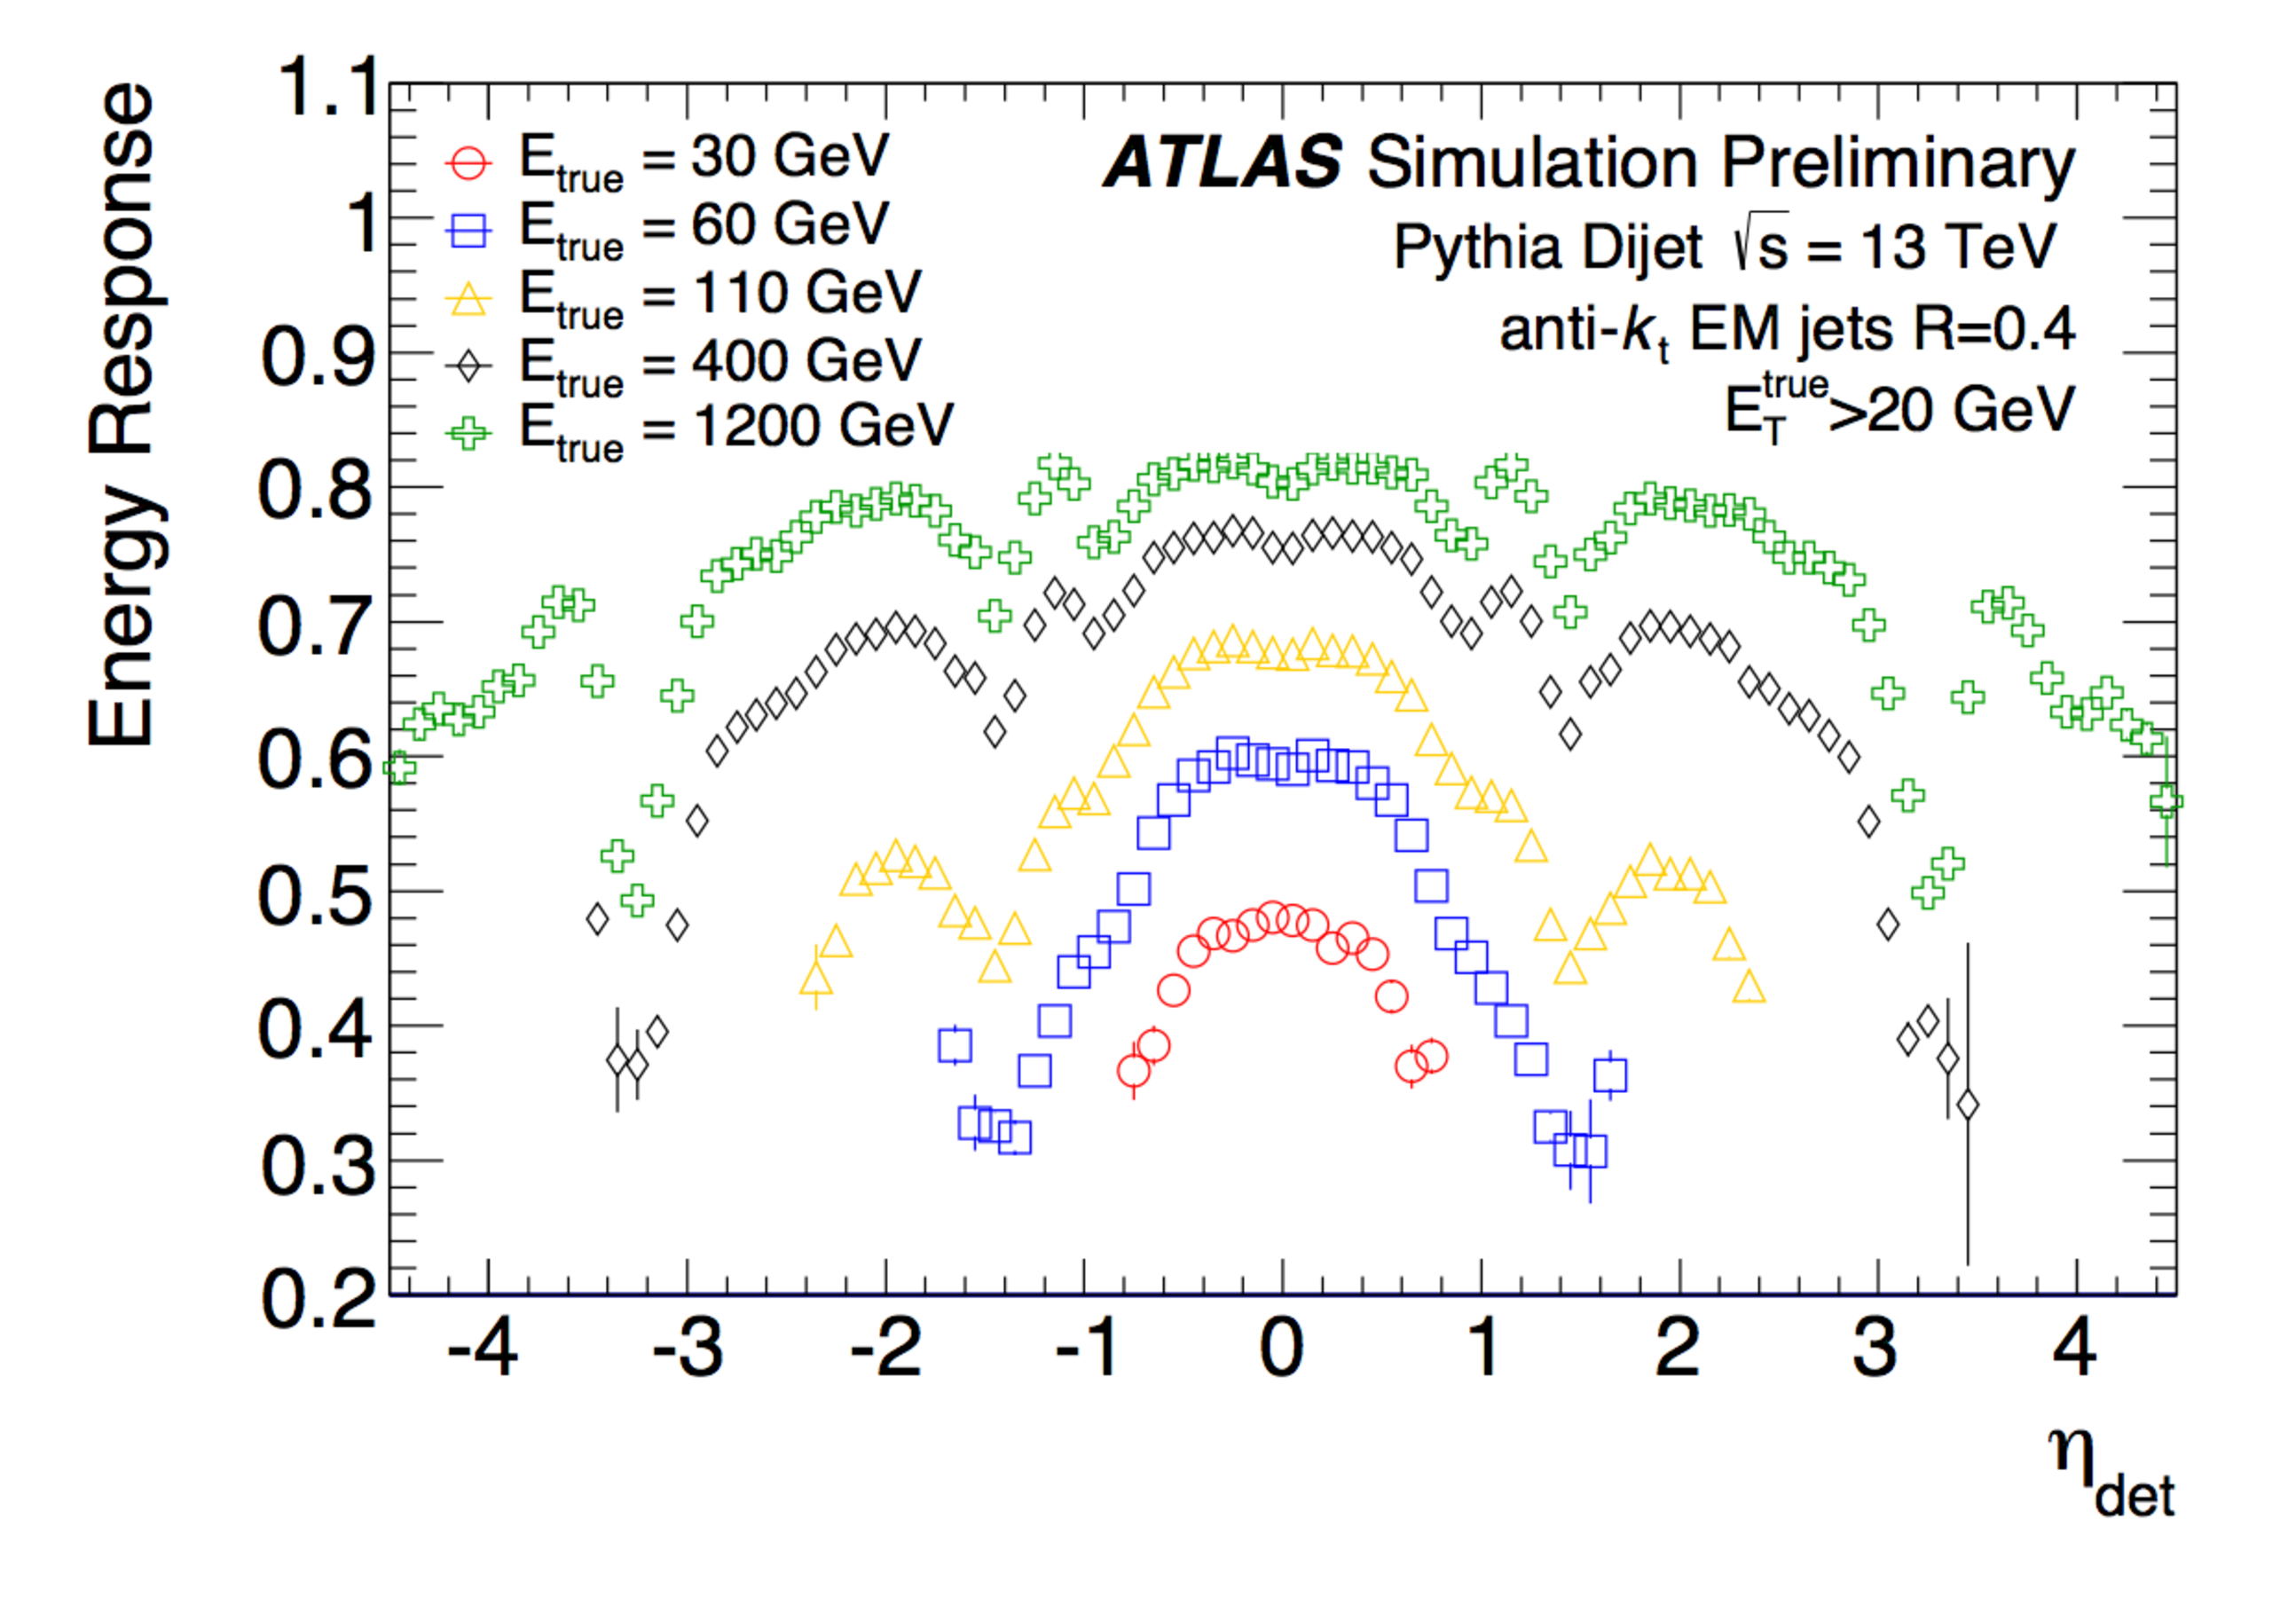
\includegraphics[width=0.48\textwidth]{figures/ObjectDef/jetResponse_pt_144.pdf}}
    \subfigure[]{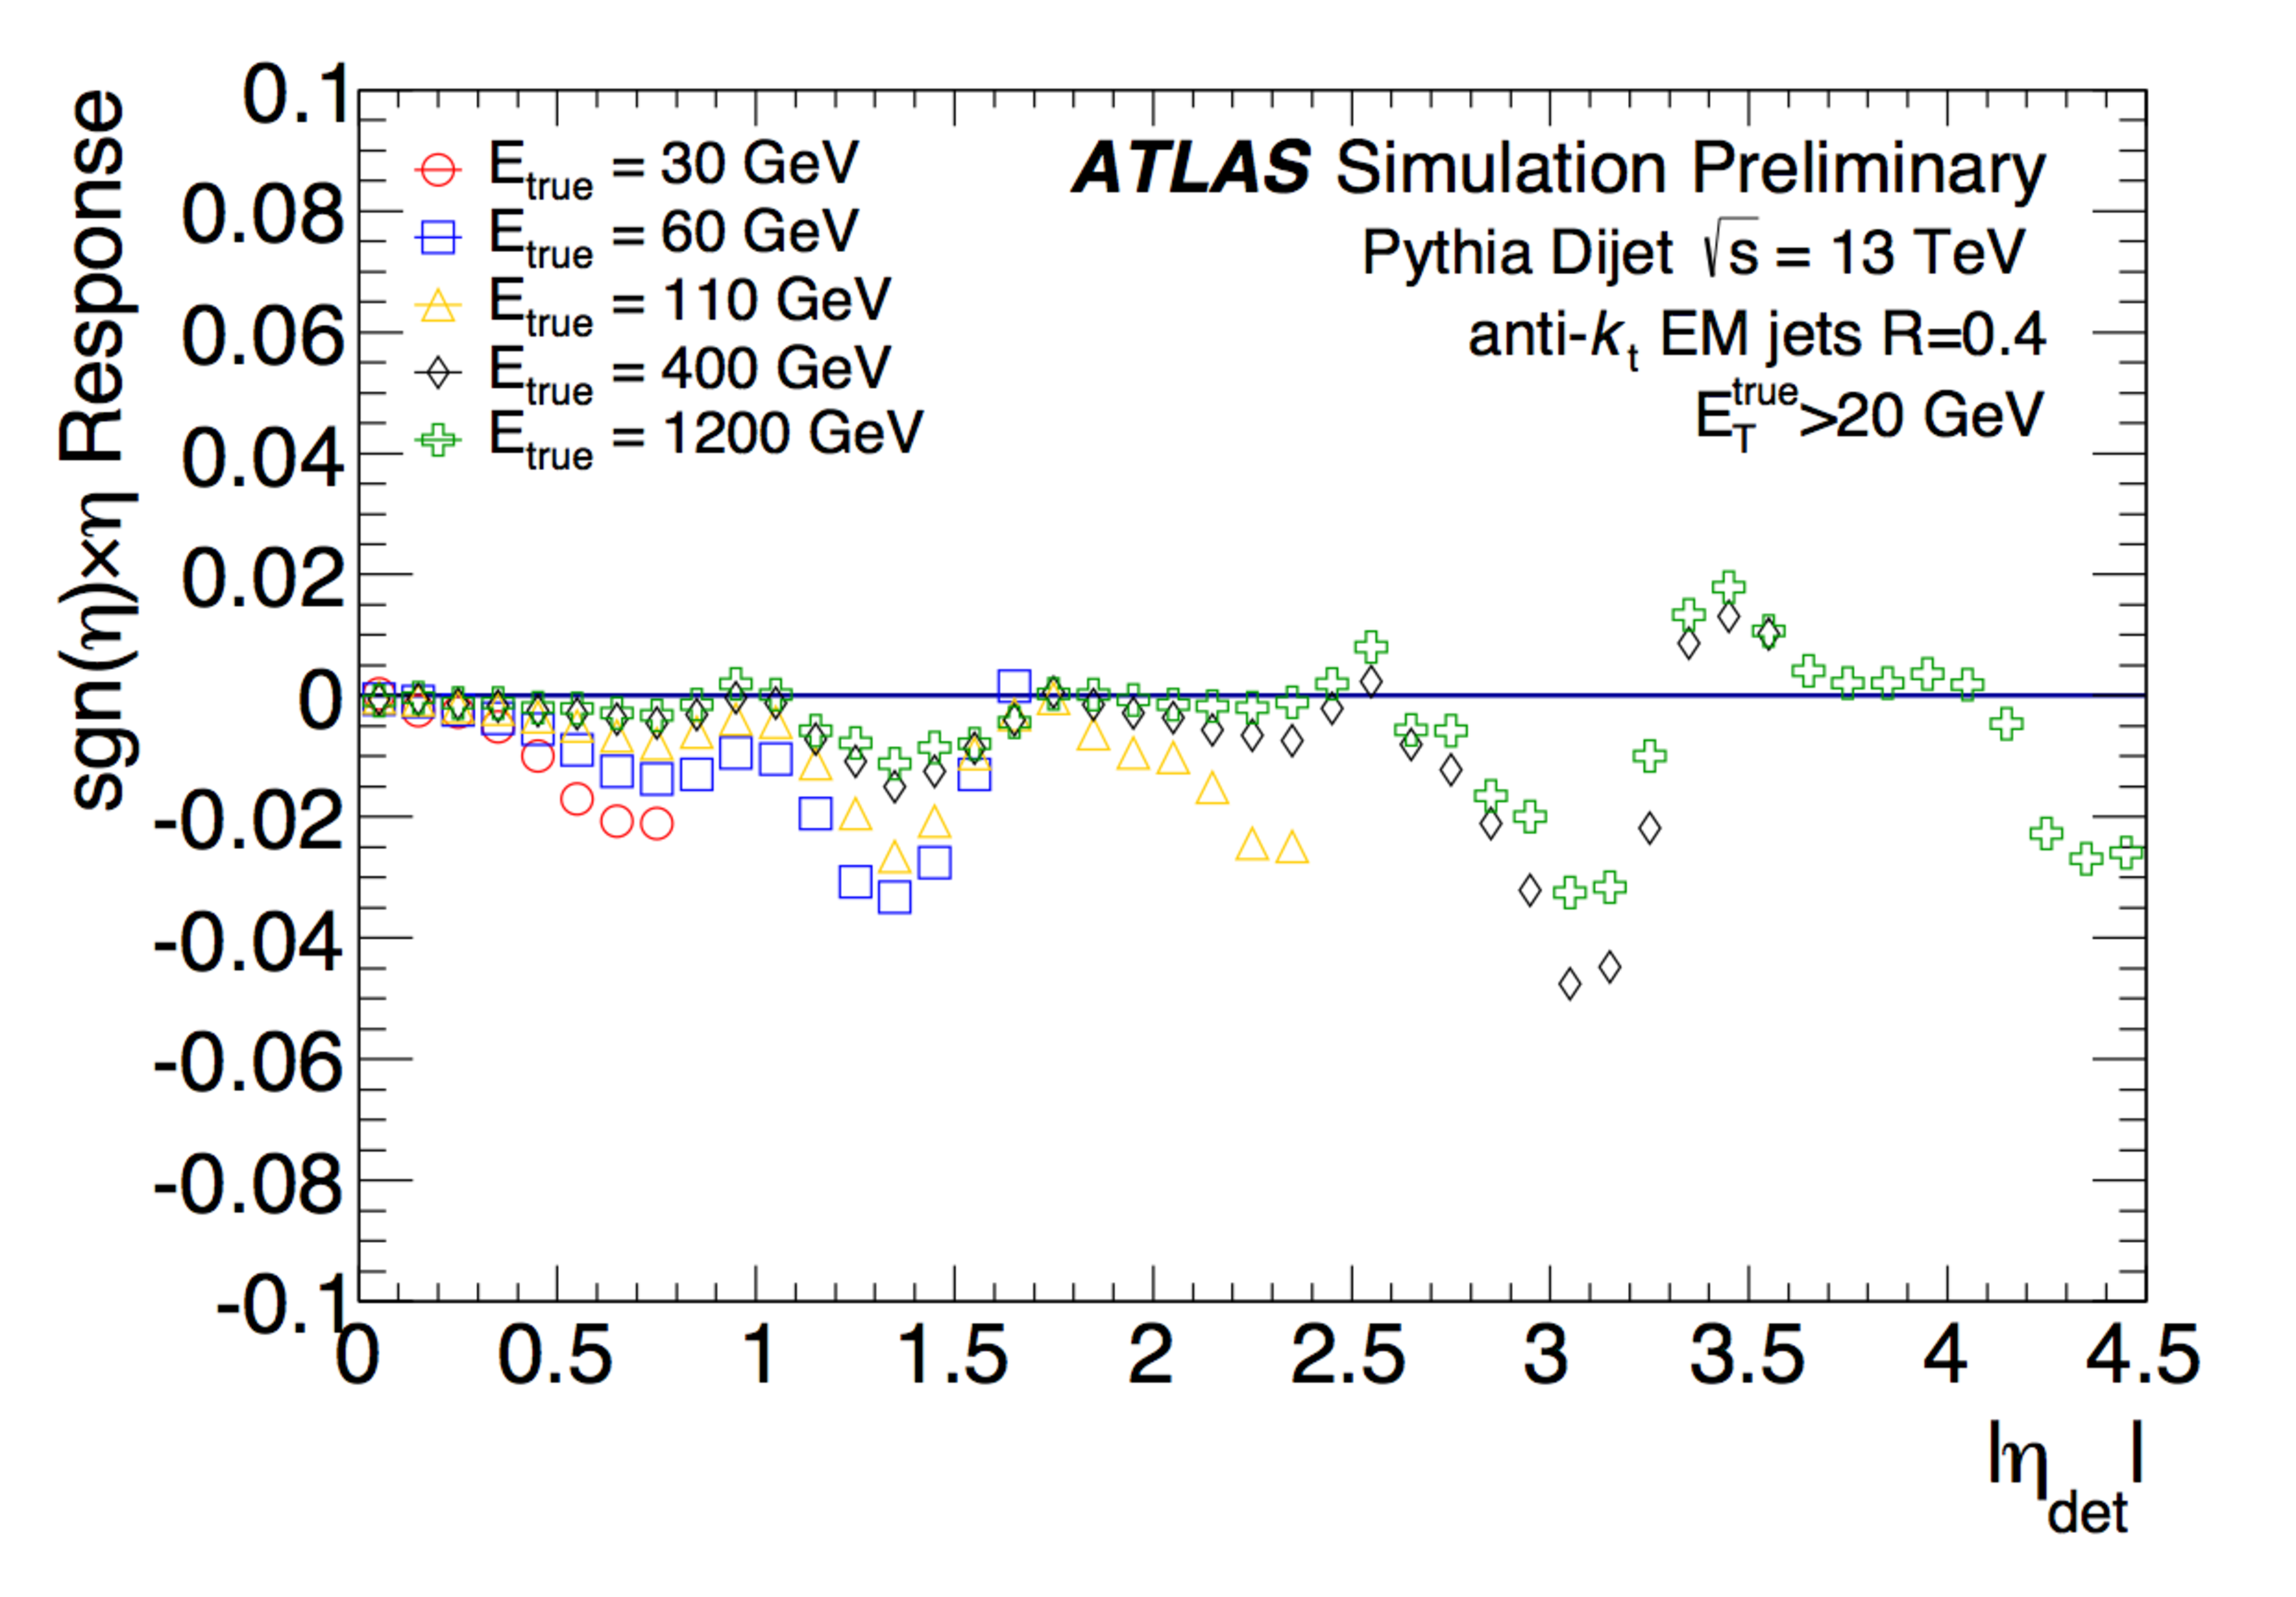
\includegraphics[width=0.48\textwidth]{figures/ObjectDef/jetResponse_eta_144.pdf}}
    \caption{ (a) Energy response and (b) $\eta$ reconstruction bias defined in Eq. \ref{eq::jetResponse} before the MC-based calibration. \cite{144_JESmeas_2015data}
      \label{fig::objDef::jetResponse} }
\end{figure}
%%%%%%%%%%





%%%%%%%%
\item \textbf{Global Sequential Calibration} \\
While only the information on topo-clusters are used for the jet energy determination so far, further improvements are achieved by applying corrections exploiting the global detector information from calorimeter, muon detector, and reconstructed tracks from inner detector. 

The procedure involves 5 independent stages, referred as the Global Sequential Calibration (GSC) \cite{140_jetEneMeas_TCcalib}, killing residual dependence of jet energy scale on the number of associated tracks or the spatial energy profile of the jet and etc. using the simulation. 

The most important function of GSC is adding robustness against varying jet flavors, in particular between quark-initiated jets and gluon-initiated, in jet energy measurement.


%%%%%%%%%%
%\begin{figure}[h]
%  \centering
%    \subfigure[]{\includegraphics[width=0.48\textwidth]{figures/ObjectDef/.pdf}}
 %   \subfigure[]{\includegraphics[width=0.48\textwidth]{figures/ObjectDef/.pdf}}
 %   \caption{ (a)  (b). 
 %     \label{fig::objDef::} }
%\end{figure}
%%%%%%%%%%




%%%%%%%%%
\item \textbf{Residual in-situ calibration} \\
A residual calibration is derived using in-situ measurements applied only to data, accounting for the differences in the jet response between data and MC simulation.
%Such differences arise from the imperfect description of the detector response and detector material in MC simulation, as well as in the simulation of the hard scatter, underlying event, pile-up, jet formation, and electromagnetic and hadronic interactions with the detector. 
The differences is quantified using data events of $\gamma+\mathrm{jet}$ and $Z\ra \mu\mu + \mathrm{jet}$,
by balancing the $\pt$ of a jet against the well-measured counterpart objects as reference.
%Similar examination are also performed on di-jets events, using the balancing technique

\end{description}



%%%%%%%%%%
\begin{figure}[h]
  \centering
    \subfigure[]{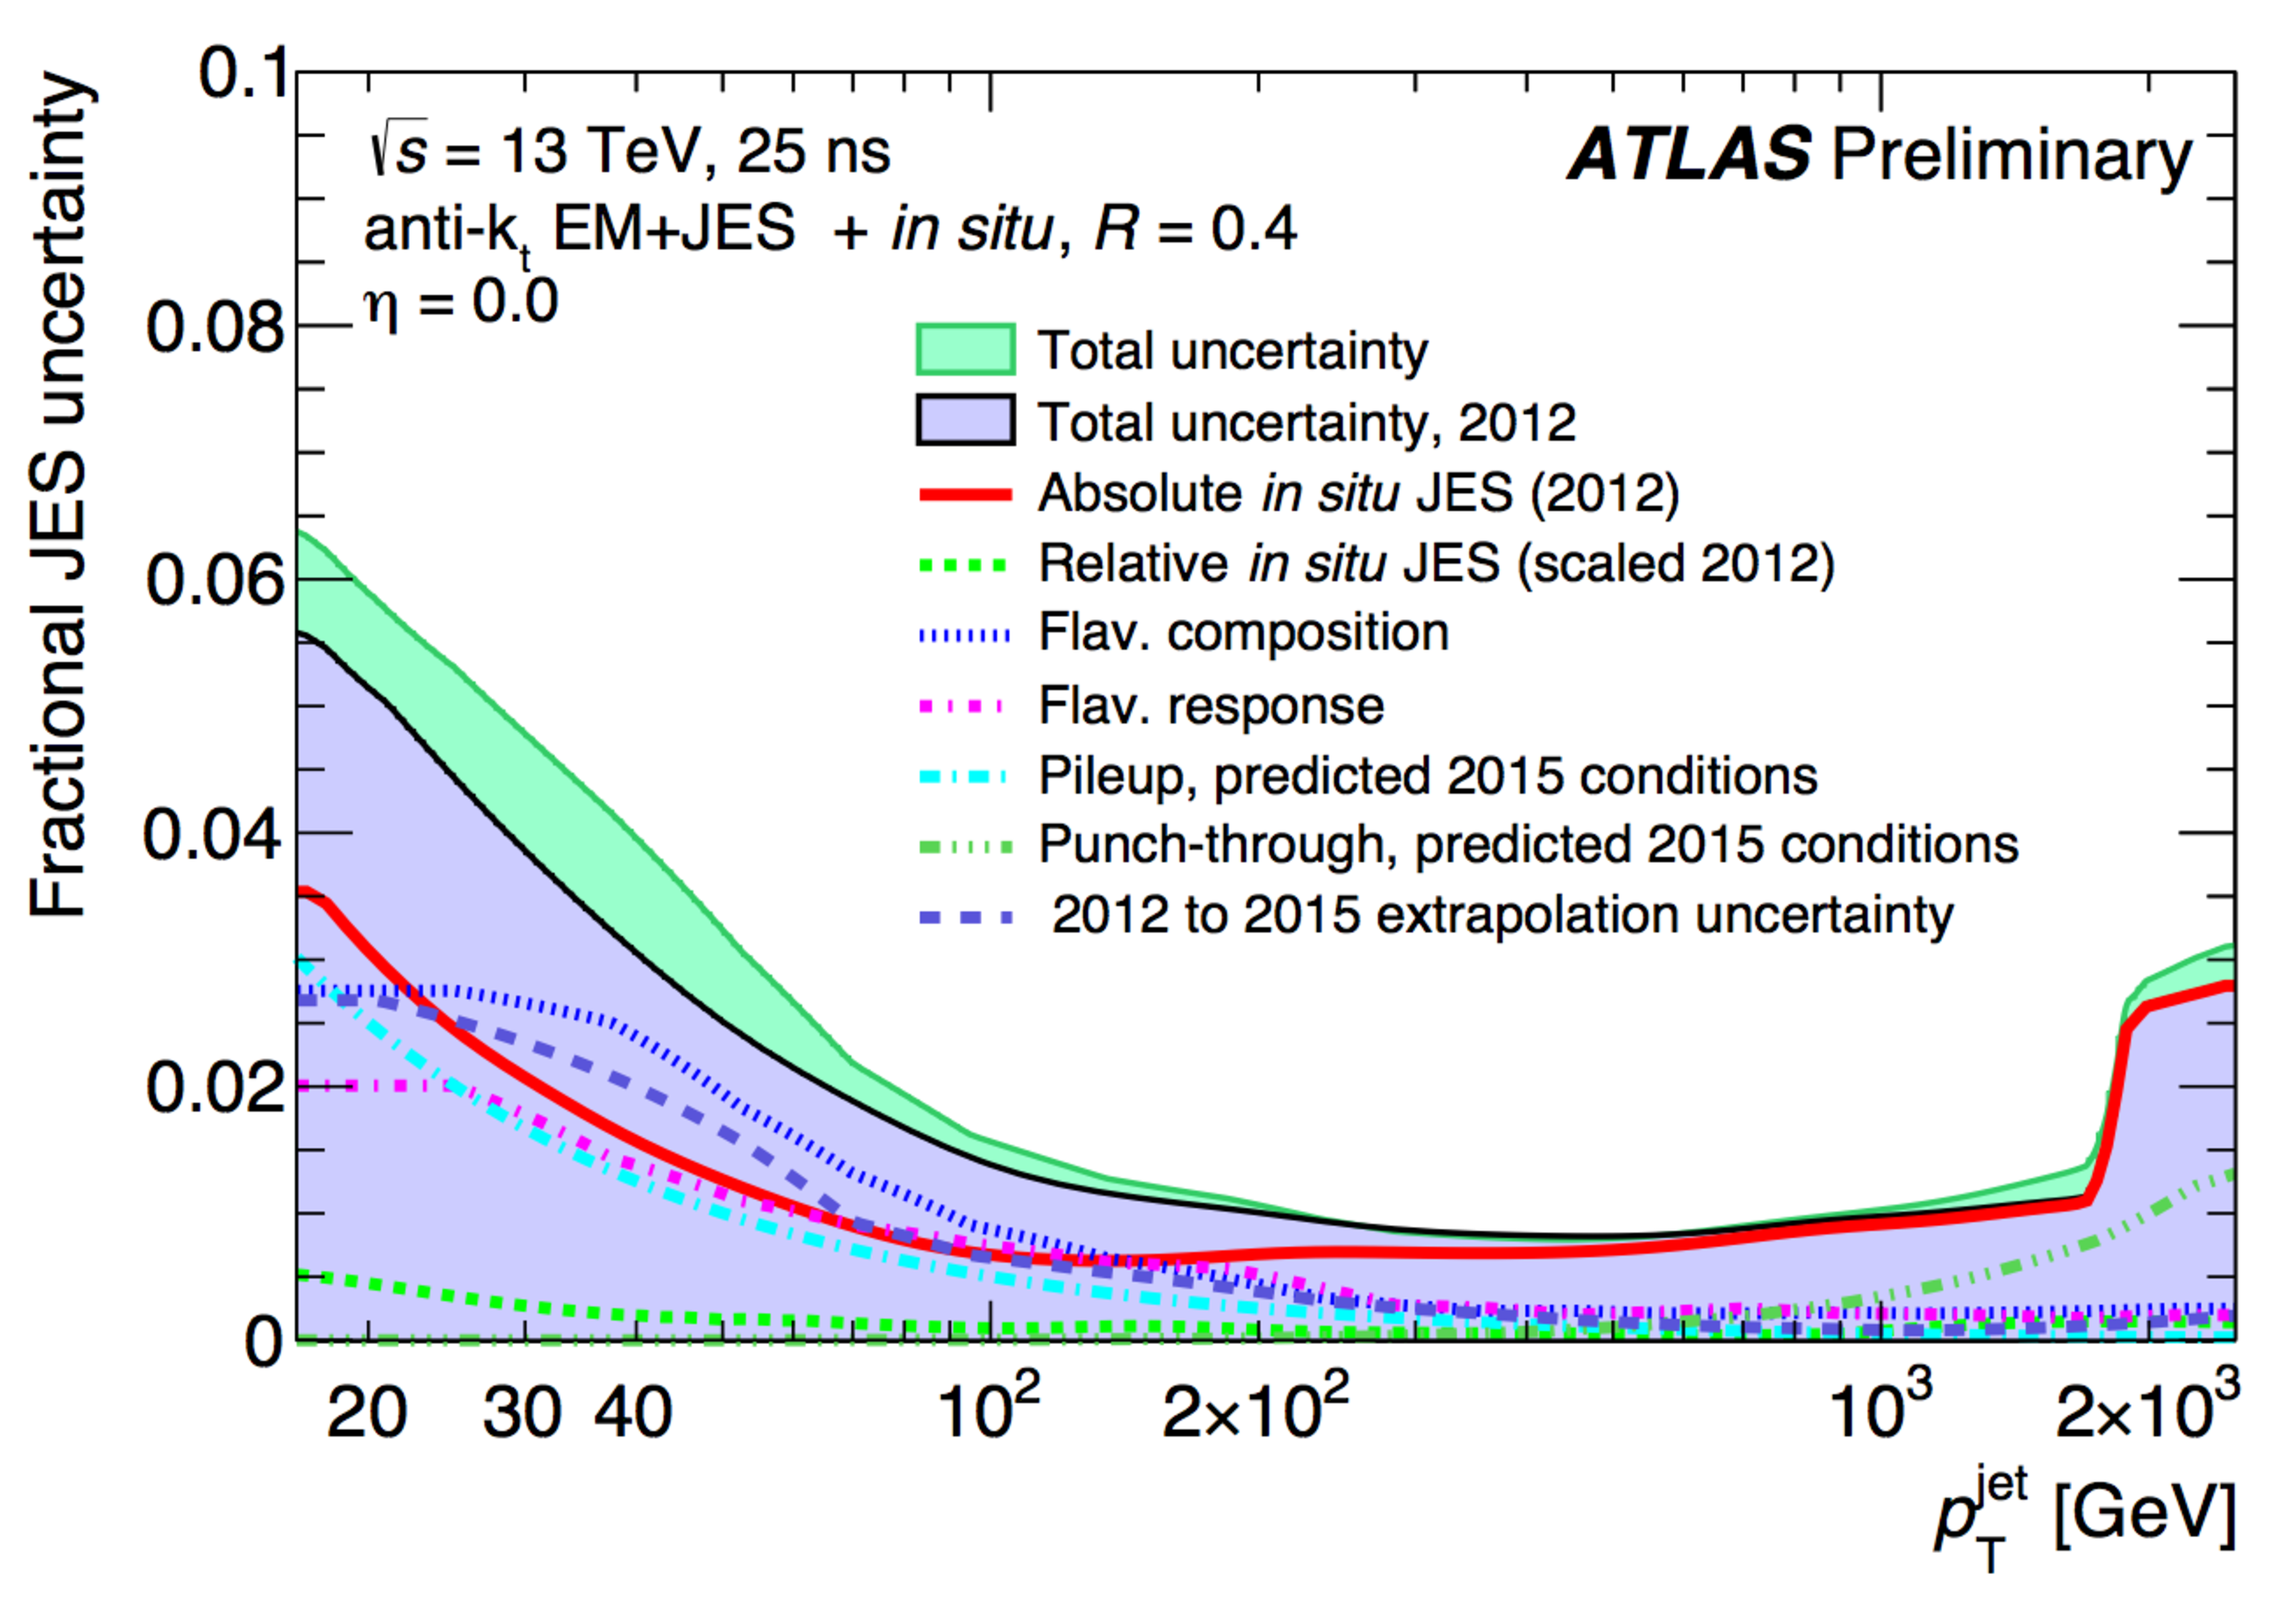
\includegraphics[width=0.48\textwidth]{figures/ObjectDef/JESUnct2015_pt_144.pdf}}
    \subfigure[]{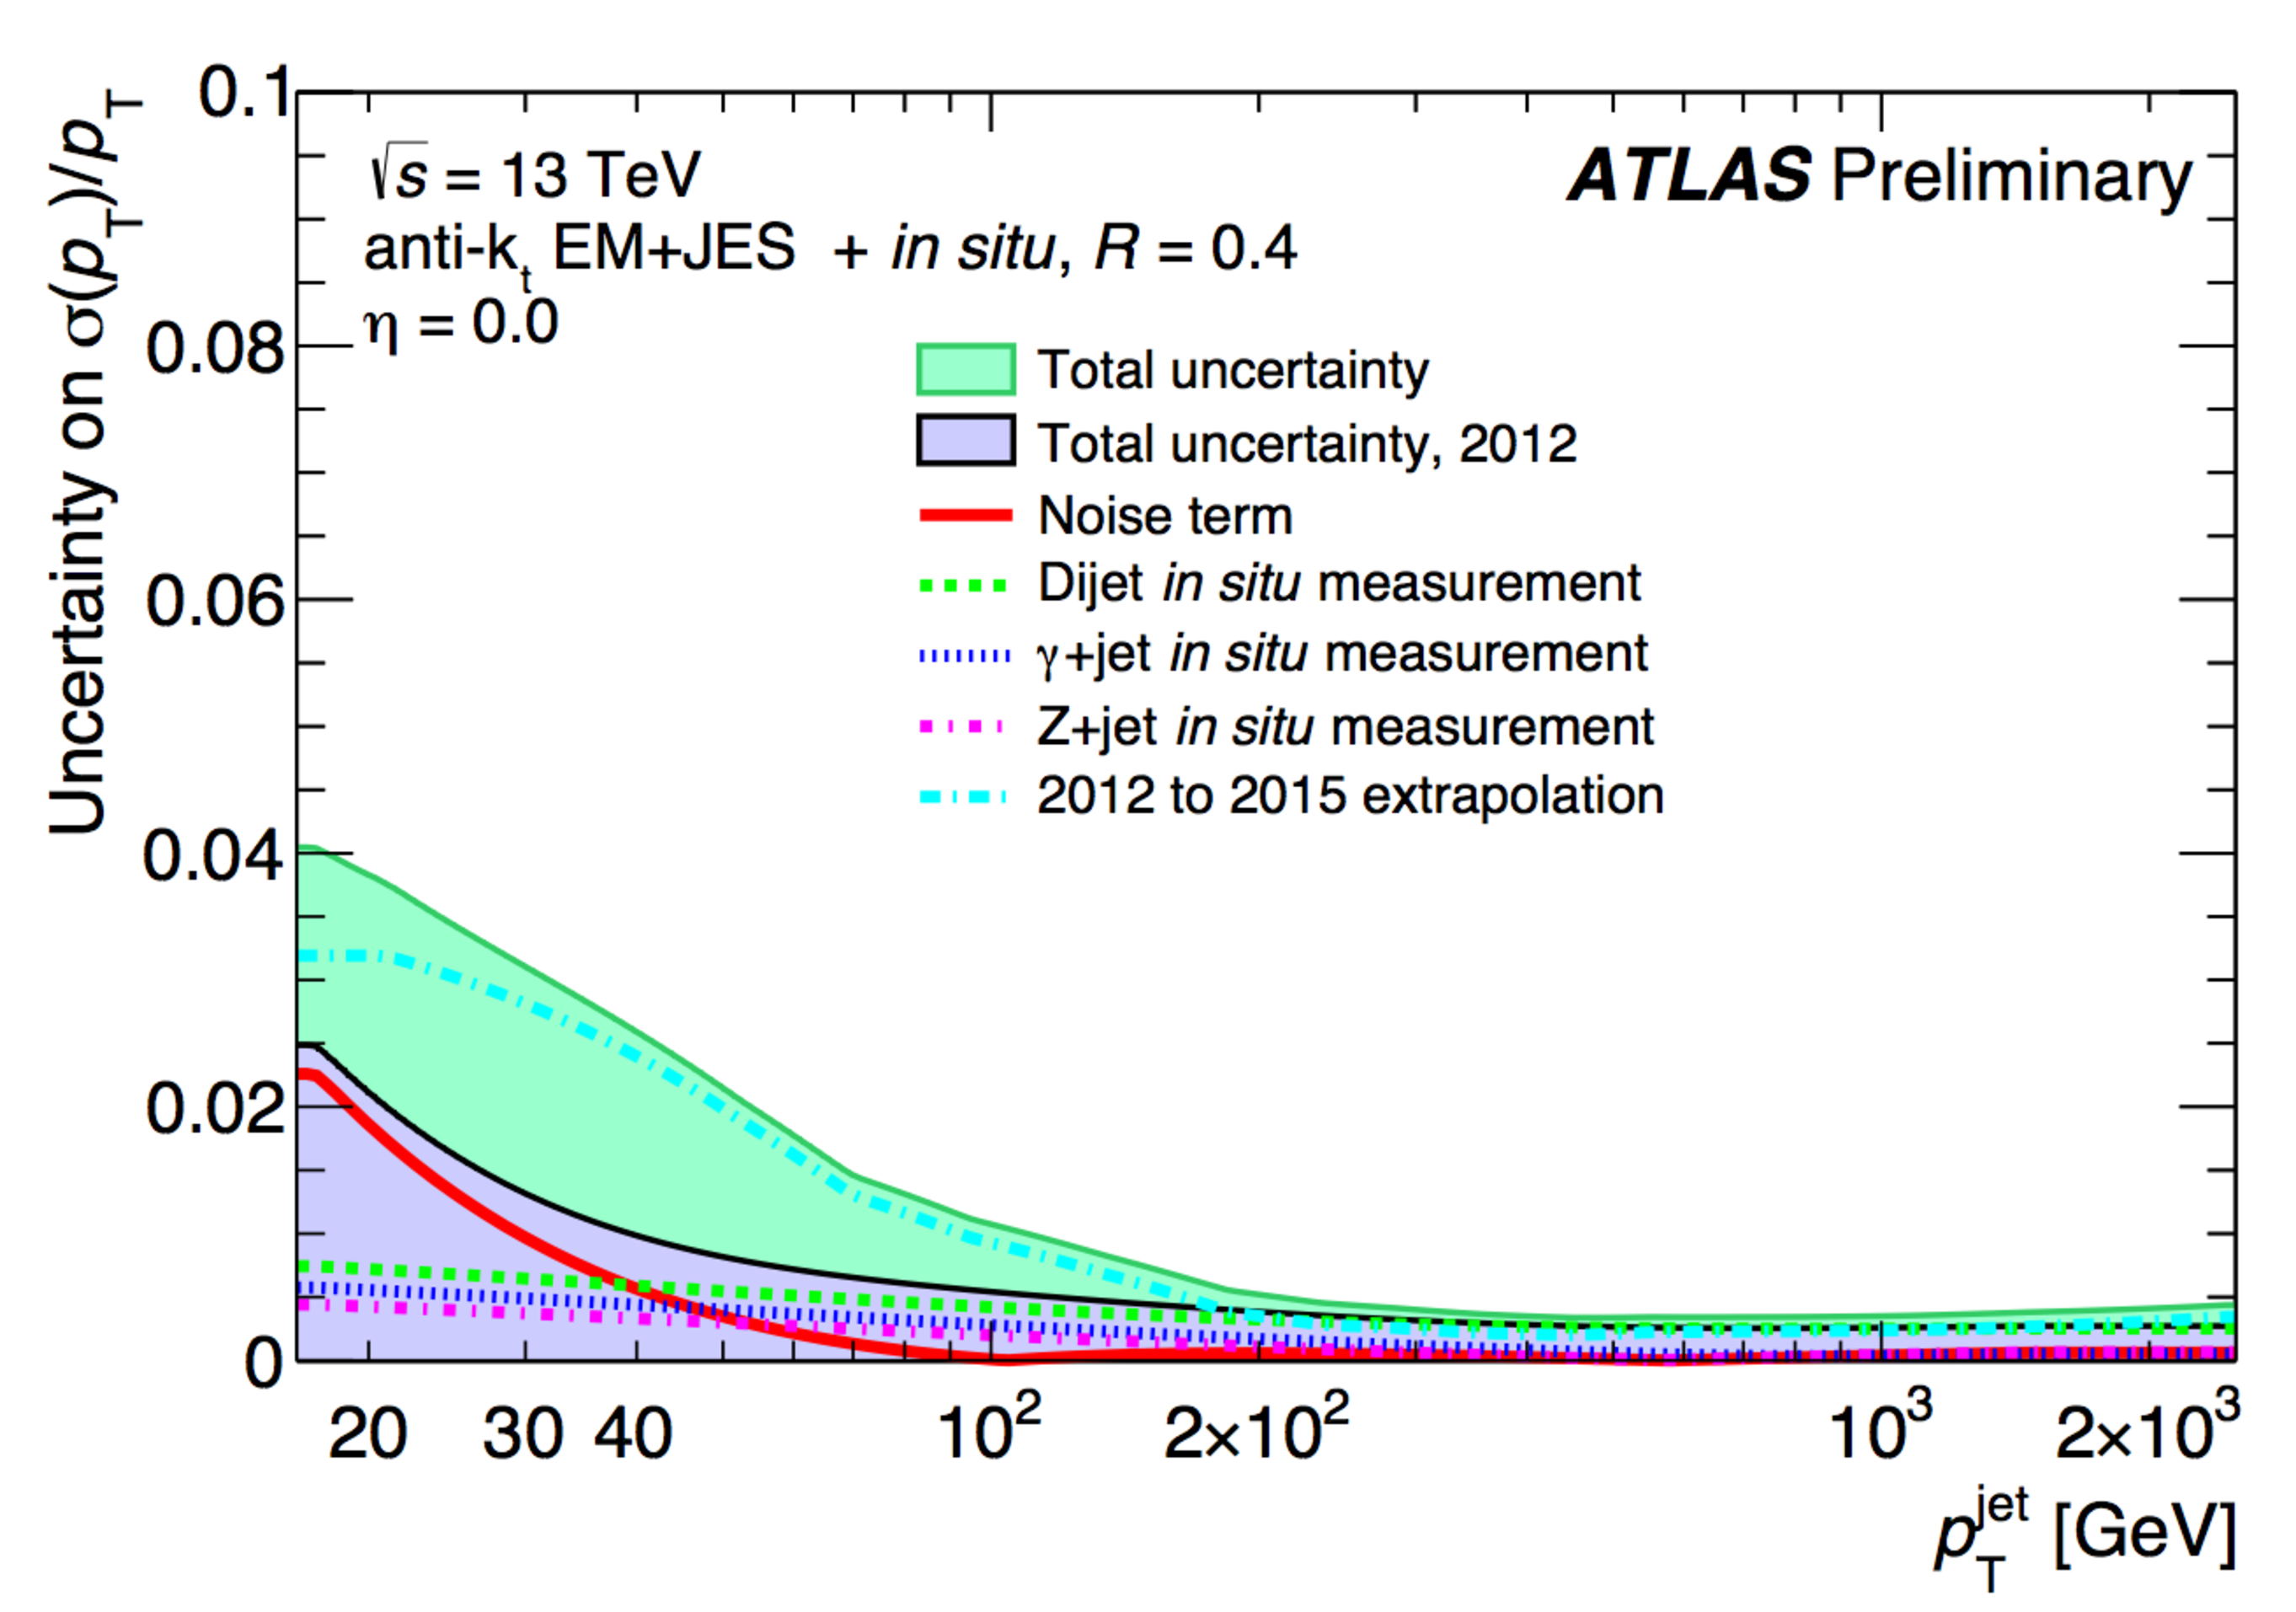
\includegraphics[width=0.48\textwidth]{figures/ObjectDef/JERUnct2015_pt_144.pdf}}
    \caption{ (a) Uncertainty on jet energy scale (JES), and (b) uncertainty on the relative resolution, with the breakdown of each sources being attached \cite{144_JESmeas_2015data}.
      \label{fig::objDef::JERUnct2015_pt_144} }
\end{figure}
%%%%%%%%%%



%%%%%%%%%
\subsubsection{B-tagging} \label{sec::objDef::jets::btag}
Hadron jets originating from $b$-quarks can be exclusively identified 
by taking advantage of the long lifetime ($c\tau\sim 450 \um$) of $b$-hadrons,
creating distinct secondary decay vertices. 
Four independent sub-algorithms (IP2D, IP3D, SV, JetFitter) exist addressing unique b-finding power. 
Their outcomes are combined by inputing them into a BDT classifier (MV2), which output is used as the final discriminant. Each sub-algorithm works as following (widely referred from \cite{150_bTag_Run2_exp} \cite{151_bTag_Run2_perf} \cite{bTag_Run2_2015data}): 

\paragraph{Impact parameter based algorithm: IP2D and IP3D}
IP2D and IP3D are the likelihood based classifiers using the impact parameter information of tracks associated to the jets. 
The track level likelihood is defined in terms of the transverse impact parameter $d_0$ and its significance $\sigma(d_0)$ (and longitudinal impact parameter $z$ for the case of IP3D), and modeled using MC respectively for the tracks in the $b$-jet and light-flavor jet. The jet-level likelihood is calculated by taking the product over all the associated tracks to the jet.
The IP2D (IP3D) is then defined by the likelihood ratio between the $b$-jet and light-flavor jet hypothesis.


\paragraph{Secondary vertex finding algorithm: SV}
The SV algorithm \cite{152_SV} explores secondary vertex finding algorithm in an explicit manner. 
After a set of qualification requirements on tracks in the jet, all the seed tracks are paired testing the consistency with the two-track vertex hypotheses. Found vertices consistent with the decays of other long-lived particles (such as $K_s$ or $\Lambda$), photon conversions or hadronic interaction with a material are rejected. As further requirements, the sum of the two impact parameter significances of the two tracks is required greater than 2, and vertices with the invariant masses exceeding $6 \gev$ are removed given the masses of the b- or c-hadrons. 
Vertex with the highest invariant mass is chosen if multiple candidates are found. %%%(要出典)


\paragraph{Decay chain multi-vertex algorithm: JetFitter}
\texttt{JetFitter} \cite{153_JetFitter} is a kinematic fittering algorithm, exploiting the topological structure of weak b- and c-hadron decays inside the jet and attempt to reconstruct the full b-hadron decay chain. Using the Kalman fitter, it finds a common line to which the PV and the bottom and charm vertices belong, approximating the b-hadron flight path, as well as their positions. The notable advantage of this approach is that the vertices of b- and c-hadron can be reconstructed, even when only a single track is attached to any of them.

\paragraph{Combinating algorithm: MV2 }
A Boosted Decision Tree (BDT) is used to combine the output from the four algorithms.
The input variables includes
the likelihood values from IP2D and IP3D,
properties of reconstructed secondary vertex (mass, position etc.) and the associated tracks providing by SV,
and the information of fitted vertices including subsequent decays of b-hadrons from JetFitter.
The full list can be found in \cite{150_bTag_Run2_exp}. \\

The output distribution and the performance is shown in Figurere \ref{fig::objDef::MV2c}.
Although the input information between the algorithms is highly correlated, the combined performance shows drastic improvement over those of either single algorithm. \\

Multiple working points are defined to provide different relative discrimination power against light-flavor jets and c-jets.
For example, MV2c10 (MV2c20) are designed to address more rejection power towards c-jets, trained using the background sample with light-flavor jets admixtured with c-jets by $10\%$ ($20\%$). 
The MV2c10 working point is used in the analysis.



%%%%%%%%%%
%\begin{figure}[h]
%  \centering
%    \subfigure[]{\includegraphics[width=0.48\textwidth]{figures/ObjectDef/.pdf}}
%    \subfigure[]{\includegraphics[width=0.48\textwidth]{figures/ObjectDef/.pdf}}
%    \caption{ (a)  (b). 
%      \label{fig::objDef::} }
%\end{figure}
%%%%%%%%%%



\fig[160]{ObjectDef/MV2c_150.pdf}
{Left plot presents the output BDT distribution for signal (b-quark jets) and backgrounds (light flavor and c-quark jets). The score of MV2c20 is shown in which c-jets rejection is reinforced.  The middle and right plot respectively show the signal efficiency vs light flavor jet rejection, and vs c-jet rejection.
 \cite{150_bTag_Run2_exp}}
{fig::objDef::MV2c}


%b-jetはsemi-leptonic decayでneutrinoが出るので通常resolutionが悪め
%calib?


%%%%%%%%%
\subsubsection{Pile-up Jet Tagging and Rejection} \label{sec::objDef::jets::JVT}
\newcommand{\pv}{\mathrm{PV}}
\newcommand{\pttk}{\pt^{\mathrm{trk}_k}}
\newcommand{\pttl}{\pt^{\mathrm{trk}_l}}
Significant fraction of reconstructed jets are originated from pile-up, particularly when they are low-$\pt$.
In order to suppress the contamination, a pile-up jet rejection is applied using the Jet Vertex Tagger (JVT) discriminant \cite{155_JVT} exploiting the vertex information.  \\

JVT is based on a 2D-likelihood function in terms of the corrected Jet Vertex Fraction (corr. JVT) and $R_{\pt}$:
\begin{align}
\mathrm{corrJVF} & := \frac{ \sum_k \pttk (\pv_0)  }{\sum_l \pttl (\pv_0) + \sum\pt(\mathrm{PU})/ (\kappa \cdot n_{\mathrm{trk}}^{\mathrm{PU}} )  }
,  \,\,\,\,\,  \sum\pt(\mathrm{PU}) = \sum_{n \ge 1} \sum_k  \pttk (\pv_n)  \nn \\
R_{\pt} & := \frac{\sum_k \pttk (\pv_0) }{\pt^{\mathrm{jet}}},
\end{align}
where $\pv_0$ denotes the hard-scatter vertex and  $\pv_j (j \ge 1)$ the other primary vertices presumably dut to the in-time pile-up interaction. 
%$n_{\mathrm{PU}}$ is the total number of pile-up tracks per event with the scaling factor $\kappa = 0.01$ determined by correlation with nl l pT (PVn) and ntrk . 
JVF (Jet Vertex Fraction) was a variable originally used for the pile-up suppression in Run1 \cite{JVF} defined by the fraction of charged tracks associated to the hard-scatter vertex:
\begin{align}
\mathrm{JVF} := \frac{ \sum_k \pttk (\pv_0)  }{ \sum_l \pttl (\pv_0) + \sum\pt(\mathrm{PU}) }.
\end{align}
While the performance of JVF is sensitive to the pileup since $\sum\pt(\mathrm{PU})$ scales linearly according to number of pileup, $\sum\pt(\mathrm{PU})$ is divided by the number of PU tracks $n_{\mathrm{trk}}^{\mathrm{PU}}$ in the corrJVF to kill the linear dependency, together with the scale factor $\kappa=0.01$ conserving the absolute normalization of the PU term.
$R_{\pt}$ is the charged energy fraction in the jet, design to address to the jets with small number of tracks leading to low corrJVF value.
A 2D-likelihood profile in terms those two variables is respectively modeled for hard-scatter jets and pile-up jets, and the JVT is defined as likehood ratio. \\

Figurere \ref{fig::objDef::JVTdist} shows the typical separation.
The JVT selection JVT$>0.57$ is applied for jets with $20 \gev < \pt< 60\gev$ and $|\eta|<2.4$, in which the pile-up jets dominantely populates.  \\


% performance, (eff, rej)
%

\fig[160]{ObjectDef/JVTdist_155.pdf}
{Left two plot display the distribution of input variables for JVT; corrJVF and $R_\phi$. corrJVF$=-1$ represents the jets with no associated tracks. The right plot is resultant output likelihood score,  JVT  \cite{155_JVT}.
}
{fig::objDef::JVTdist}

%\fig[80]{ObjectDef/JVTeff_155.pdf}
%{JVTeff. \cite{155_JVT}}
%{fig::objDef::JVTeff}



%%%%%%%%%%
%\begin{figure}[h]
%  \centering
%    \subfigure[]{\includegraphics[width=0.48\textwidth]{figures/ObjectDef/.pdf}}
%    \subfigure[]{\includegraphics[width=0.48\textwidth]{figures/ObjectDef/.pdf}}
%    \caption{ (a)  (b). 
%      \label{fig::objDef::} }
%\end{figure}
%%%%%%%%%%



%%%%%%%%%
\subsection{Overlap Removal between Reconstructed Objects} \label{sec::objDef::OR}
Electrons, muons and jets are reconstructed in parallel, allowing the ambiguity that an identical particle is reconstructed or identified as multiple types of particles simultaneously. 
For instance, electrons are typically reconstructed either as electrons and jets. 
This is designed to provide flexibility in the object definition to satisfy various needs by analyses.  \\

A sequence of ``overlap-removal'' procedure is applied to resolve the ambiguity and avoid the double-counting, based on the angular distance $\Delta R = \sqrt{\eta^2+\phi^2}$ between them.  \\

The algorithm begins with the electron-jet overlap removal.
Any light-flavor jet \footnote{defined as reconstructed jets with b-tagging score MV2c10$<0.1758$ which corresponds to $85\%$ effciency for real b-jets.} 
reconstructed within $\Delta R < 0.2$ with respect to identified electrons is rejected.
The electron is otherwise removed if the overlapping jet is b-tagged jet, 
to avoid rejecting b-jets due to the non-prompt lepton nearby caused by the decays of b-hadrons. Next, to remove bremsstrahlung from muons followed by a photon conversion into electron pairs, electrons lying within $\Delta R < 0.01$ of a preselected muon are discarded.  \\

Subsequently, the contamination of muons from heavy-flavored hadron decays is suppressed by removing muons that lie within $\Delta R < \min(0.04 + (10 \gev)/\pt, 0.4)$ of any remaining jet, or within $\Delta R < 0.2$ of a b-tagged jet or a jet containing more than three tracks with $\pt > 500 \mev$.
In the former case, the $\pt$-decreasing angular separation mitigates the rejection of energetic muons close to jets in boosted event topologies. Finally, jets reconstructed within $\Delta R < 0.2$ of remaining electrons or muons are excluded. \\

The identification of hadronically decaying taus and photons are not exploited in the analysis, since they are not explicitly used as objects in event selections. Instead, those with sufficiently high transverse momentum pass the jet reconstruction as well as the JVT requirement, thus treated as jets in the analysis. \\
%%% table?


%%%%%%%%%
\subsection{Fake Leptons and the Isolation Requirement} \label{sec::objDef::fakeAndIsolation}
Light flavor leptons (electrons or muons) produced in LHC subject to two types; ``prompt leptons'' directly originated from the hard scattering via decays of real and virtual gauge bosons; ``non-prompt leptons'' generated via decays of heavy flavor hadrons (contains $b$ or $c$ quarks) and tau leptons, or pair creation of photons (mostly stemming from $\pi_0$ in jets). The leptons interested in the new physics or EW physics always always refer to the prompt leptons, while non-prompt leptons are trivial and disturbing, degrading the use of leptons in the analysis. There are also a type of reconstructed leptons by wrongly identified pions from jets. In the thesis, these unwilling kinds of leptons (non-prompt leptons and pions) are simply referred as ``fake lepton'', and suppressed by employing the extra requirement described as follows.

\paragraph{Impact parameter requirement}
Non-prompt leptons are generated in relatively displaced position with respect to the primary vertex. Therefore, the information of transverse impact parameters address a nice discriminating power. The selection used in the analysis is as Table \ref{tab::ObjDef::impactPar}.
While the $d_0$ and $|z_0 \sin{\theta}|$ of prompt-leptons populate close to 0, those fornon-prompt leptons result in wide distributions, leading many of them to be rejected.

\tab{c|c|c}
{
\hline
                                     &   Electron &   Muon \\
\hline
\hline
$|d_0/\sigma_{d_0}|$                 &   $<5$       &   $<3$   \\
$|z_0 \sin{\theta}|$   &   $<0.5$ mm     &   $<0.3$ mm  \\
\hline
}
{
Summary of impact parameter requirements used in the analysis. 
$d_0$ and $z_0$ is the transverse and longitudinal impact parameter respectively.
$\sigma_{d_0}$ is the defined by the error matrix of the track fit
}
{tab::ObjDef::impactPar}

%%% fig?


\paragraph{Isolation}
While the path of flight of prompt-leptons rarely overlap with other particles, fake leptons generally fly closely by jets for their origin. Relatively higher jet activity around fake leptons is expected, therefore the isolaton requirement with respect to proximate cluster or tracks provide significant rejecting power of fake leptons. \\

Two isolation variables are defined:

\begin{description}
\item {\textbf{Calorimeter isolation} ($\etcone$)}: Sum of transverse energies by the calibrated topo-clusters 
with  $\Delta R<0.2$ with respect to the lepton. An $\et,\eta$ dependent pileup correction is applied. For electron, the energy leakage due to the bremstralung is compensated. 

\item {\textbf{Track isolation} ($\ptcone$)}: Sum of transverse momentum of tracks within the angular distance of $R=\min(0.2, 10\gev/\pt)$ with respect to the lepton. The variable cone size is intended to loosen the isolation cut for high-$\pt$ leptons, based on the fact that most of fake leptons are below $20\gev$.
\end{description}

The isolation requirement is done by applying a cut in a 2D-plane of $\etcone$ and $\ptcone$. 
In the analysis, the \texttt{GradientLoose} working point is chosen, in which a $\pt$-dependent cut is applied designed to recover the efficiency in high-$\pt$. Figurere \ref{fig::objDef::isoEff}  shows the isolation efficiency respectively for electrons and muons. \\

%%%%%%%%%%
\begin{figure}[h]
  \centering
    \subfigure[]{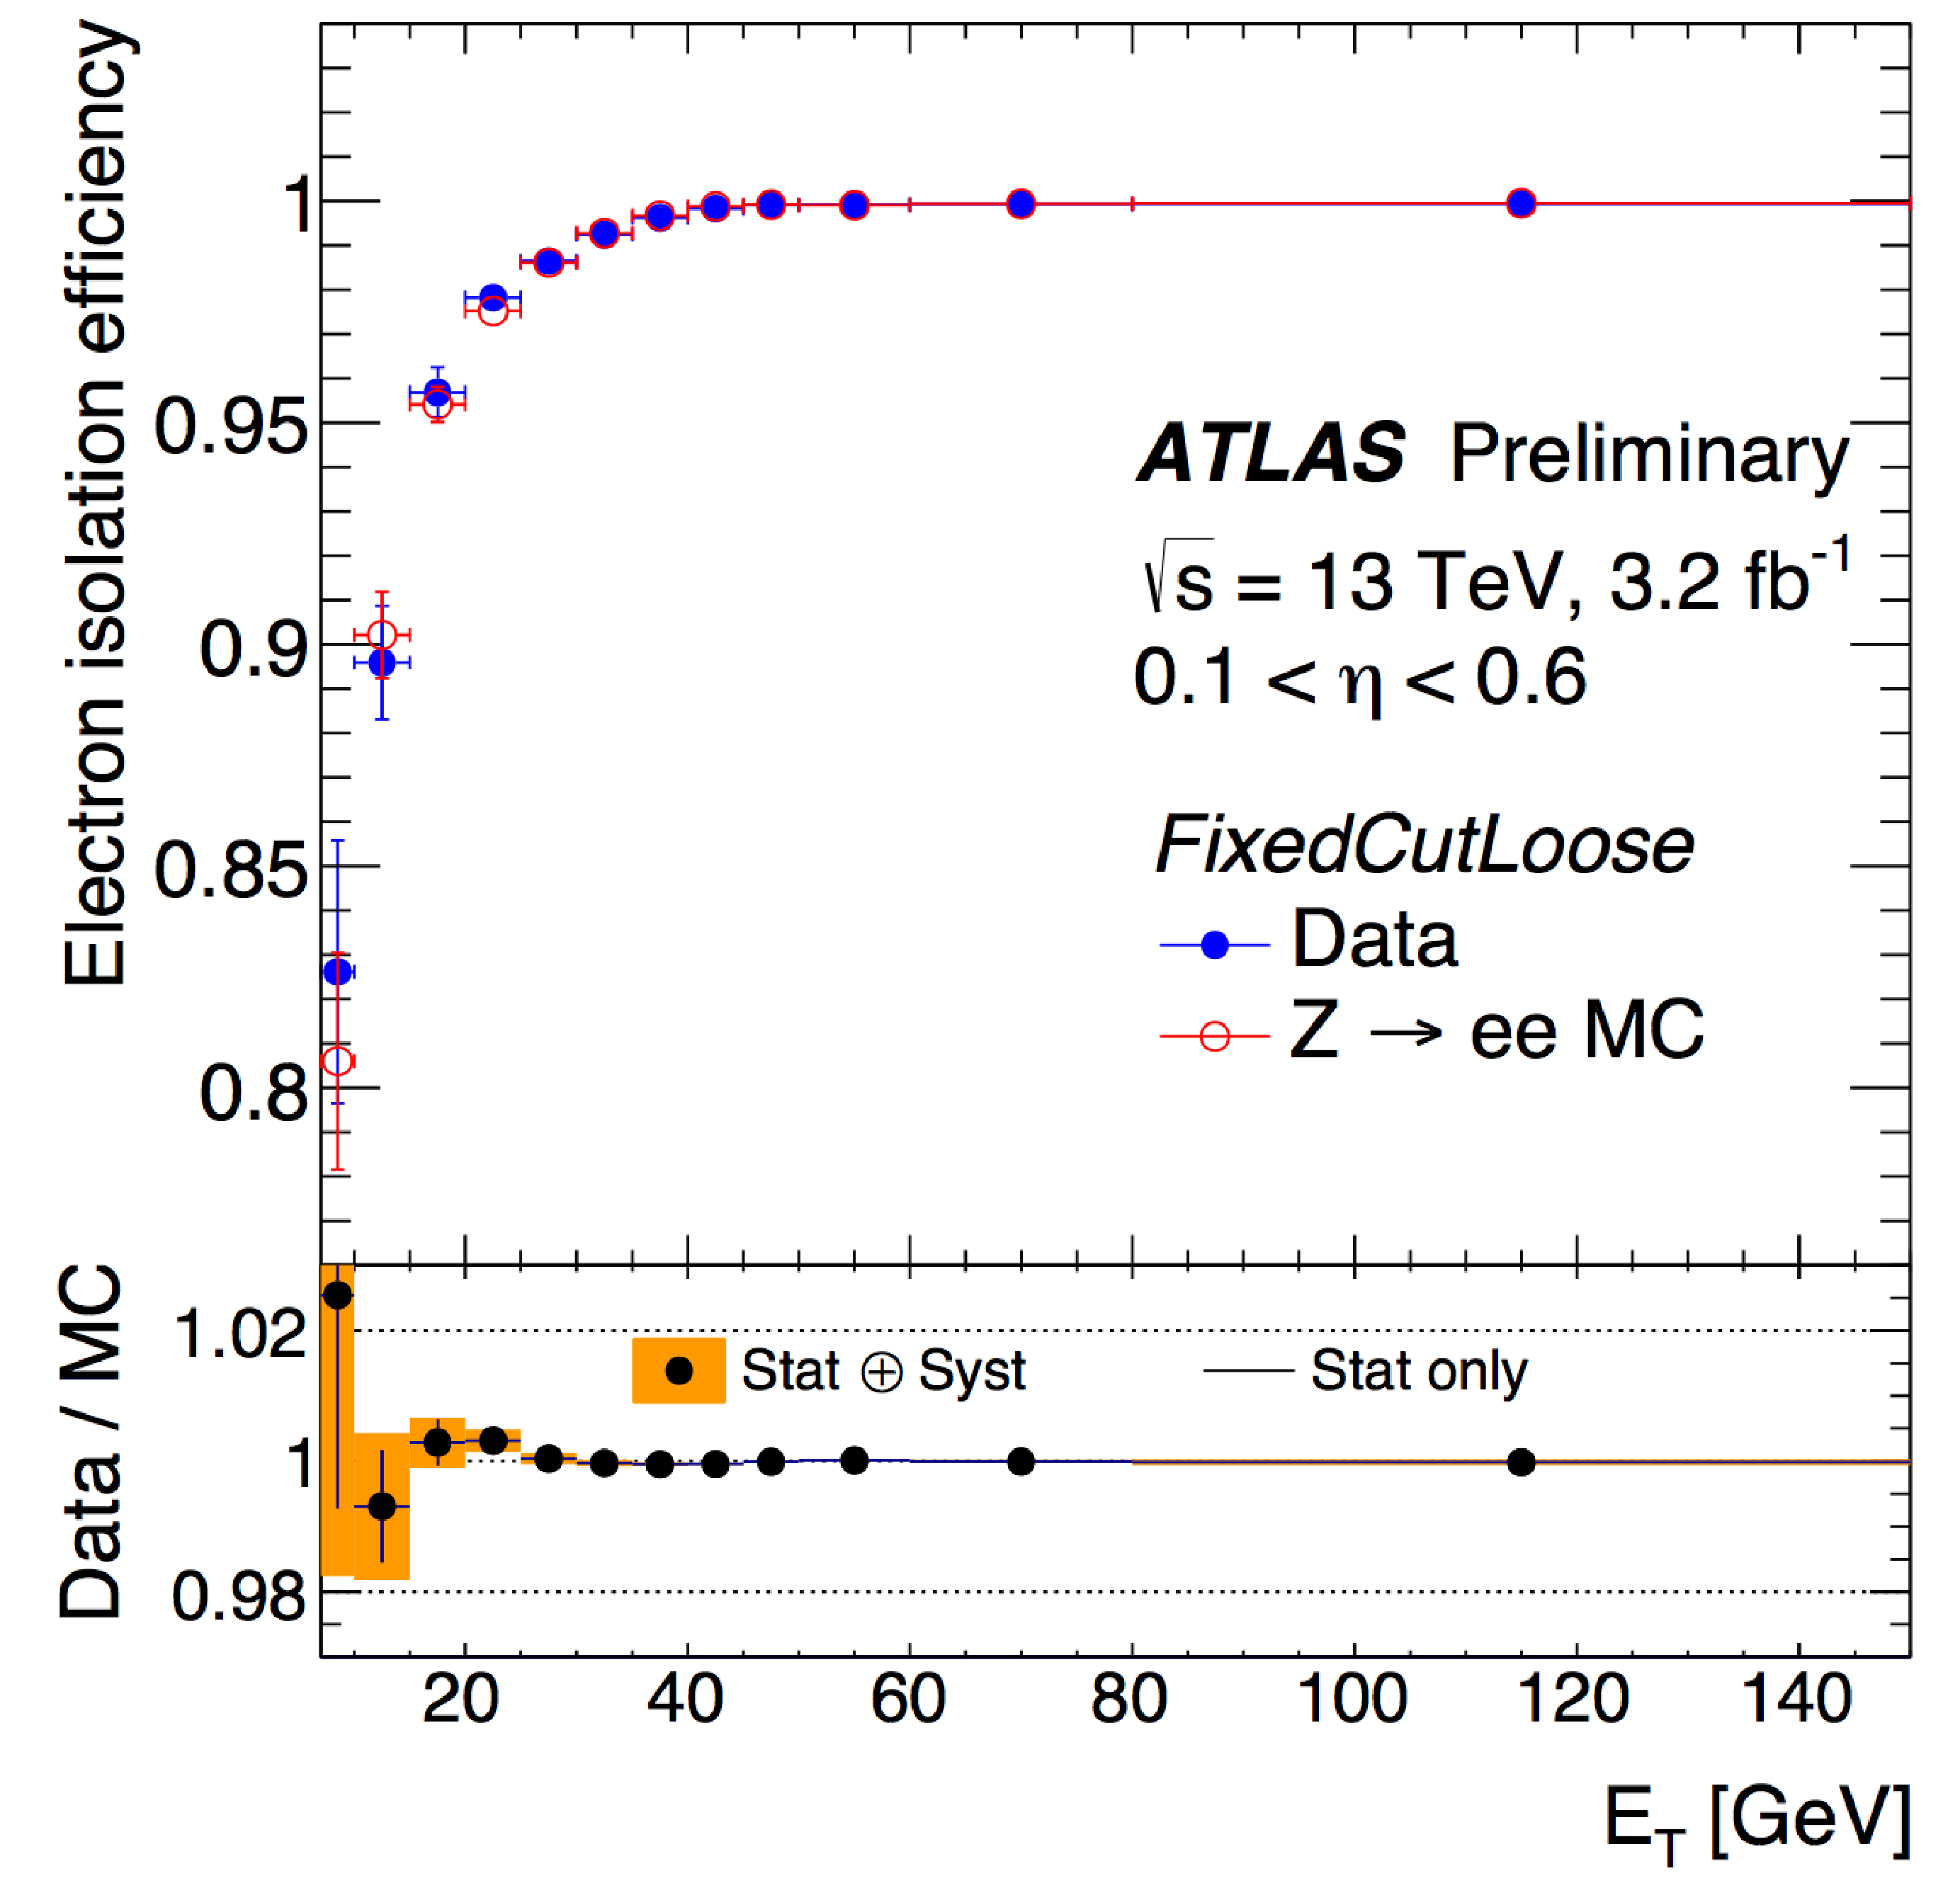
\includegraphics[width=0.48\textwidth]{figures/ObjectDef/electronIsoEffFixedCutLoose_pt_156.pdf}}
    \subfigure[]{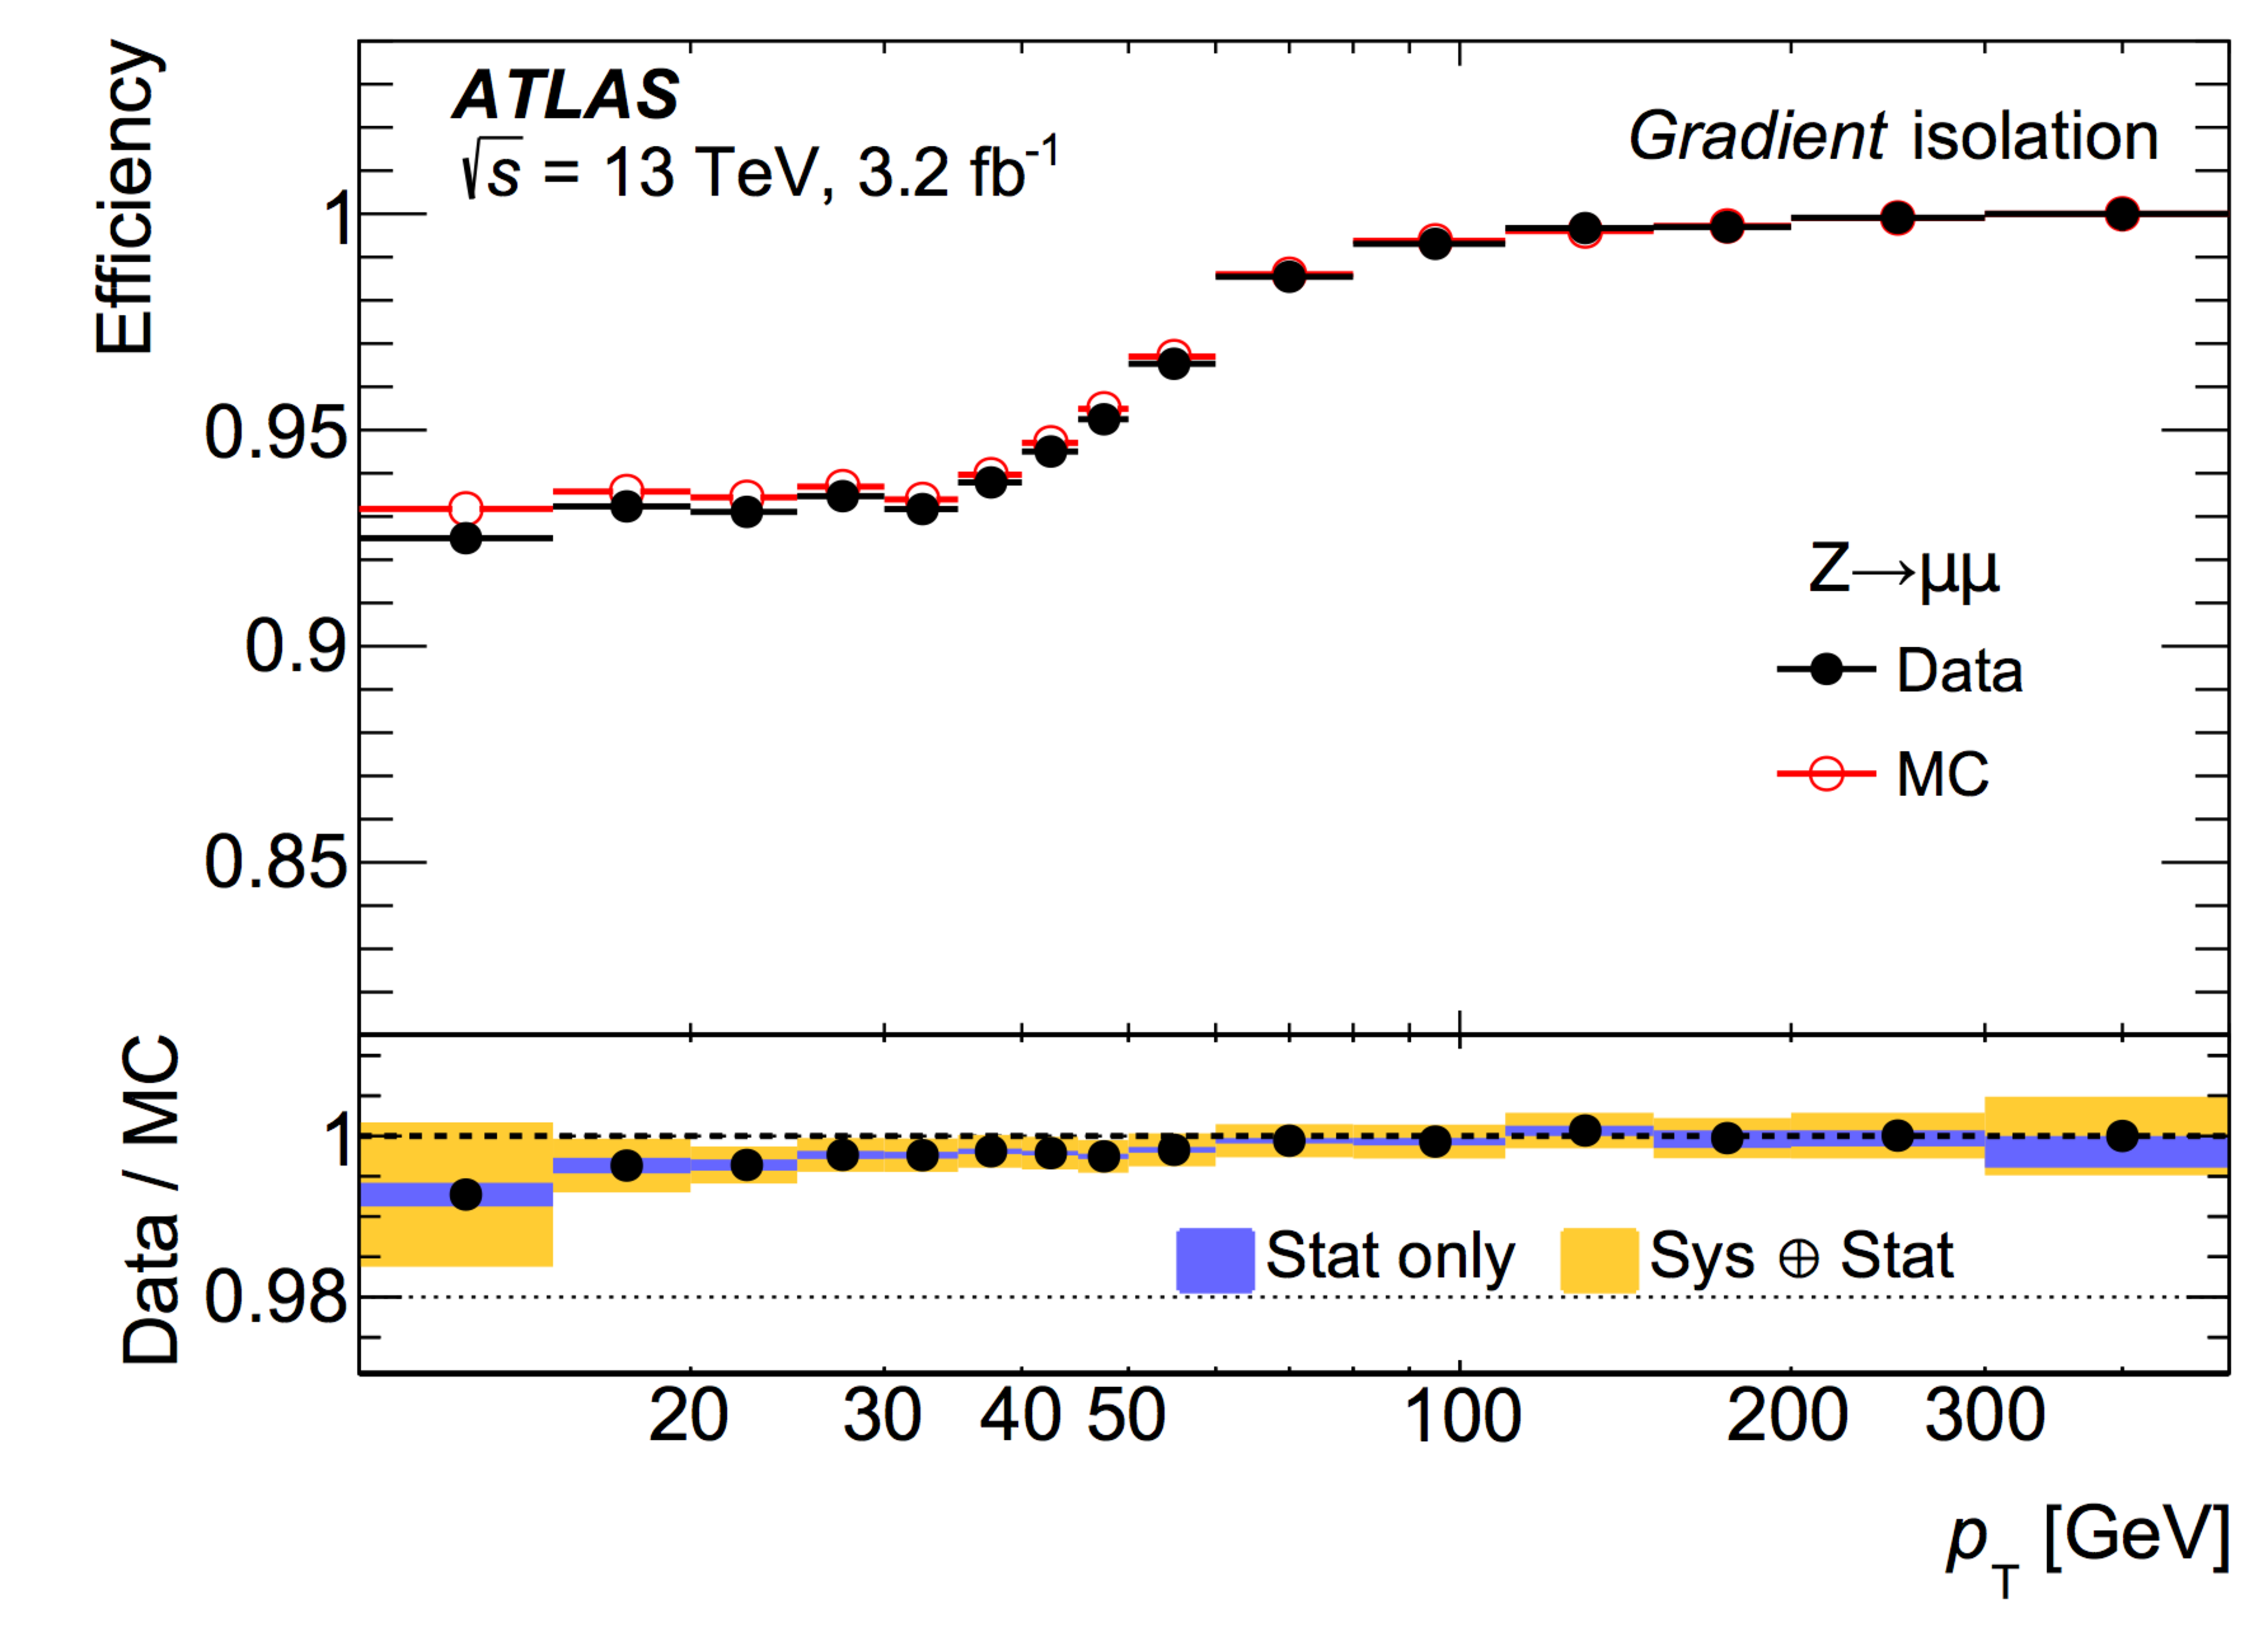
\includegraphics[width=0.48\textwidth]{figures/ObjectDef/muonIsoEffGradLoose_166.pdf}}
    \caption{ Measured and expected efficiency for isolation requirement for (a) electrons\cite{156_ElectronEffMeas_2015data} and (b) muons \cite{166_muonPerformance2015data}, both using the $Z\ra ee/\mu\mu$ events.
      The \texttt{FixedCutLoose} working point is shown for the electrons where $\etcone/\ET<0.2$ and $\ptcone/\ET$<0.15 is applied.
      \label{fig::objDef::isoEff} }
\end{figure}
%%%%%%%%%%



%%%%%%%%%%%%%%%%%%%%%%%%%%%%%%%%%%%%%%%%%%%%%%%
\subsection{Missing Transverse Energy} \label{sec::objDef::met}
Missing Transverse Energy ($\met$) is an extremely important proxy to new physics since it is contains the kinematical information of invisible particle. $\met$ is calculated by the transverse momentum imbalance of visible particles, using the reconstructed objects as well as isolated tracks that does not associated to any reconstructed objects referred as the soft term.
It is contructed by four independent terms as shown in Eq. (\ref{eq::metDef}):
\begin{align}
\bm{E_\mathrm{T}^{\mathrm{miss.}}} :=  - \sum \bmet^{e} - \sum \bmet^{\mu} - \sum \bmet^{\mathrm{jet}} - \bmet^{\mathrm{soft}}.
%\met_{x,y} :=  - \sum \ET^{e}_{x,y} - \sum \ET^{\mu}_{x,y} - \sum \ET^{\mathrm{jet}}_{x,y} - \sum \ET^{\mathrm{soft}}_{x,y}.
\label{eq::metDef}
\end{align}
Input reconstructed objects for the first three terms in Eq. (\ref{eq::metDef}) are fully calibrated and the ambiguity between them is resolved by the overlap removal. 
%The overlap removal procedure used for $\met$ calcualtion slightly differes from the baseline method described in the previous sub-section in that  (要確認)
Jets with $\pt>20\gev$ are included in the jet term in the MET calculation, otherwise subjected to the soft term with the track momenta.
%unique fraction
Jets failed in the JVT selection is totally excluded from the MET calculation to prevent the contribution from pile-up. \\

The track soft term $\bmet^{\mathrm{soft}}$ (TST) \cite{175_MET_Run2_exp} accounts for the residual visible momentum mainly from soft jets and unidentified muons.
It is constructed by the tracks that are not associated to any jet, and are isolated by $\Delta R>0.2$ from any reconstructed EM clusters. The momenta of tracks found to associated with reconstructed muons are replaced into that by the combined ID+MS muon tracks. 
Tracks has its track momentum uncertainties larger than $40\%$, and high-$\pt$ tracks ($\pt>200 \gev$ in $|\eta|<1.5$ or $\pt>150 \gev$ in $|\eta|>1.5$) with questionable quality of monemtum measurement satisfying following conditions are removed to prevent potential large error in the calculation:
\begin{align}
\ptcone/\pt>0.1, \,\,\, \mathrm{and} \,\,\, \frac{\etcone}{\pt+\ptcone}<0.6, \,\,\,  \mathrm{and} \,\,\, \frac{\ptcone}{\pt+\ptcone}<0.6
\end{align}
% isolation variable defined in previous sub-section


%%%%%%%%%%
\begin{figure}[h]
  \centering
    \subfigure[]{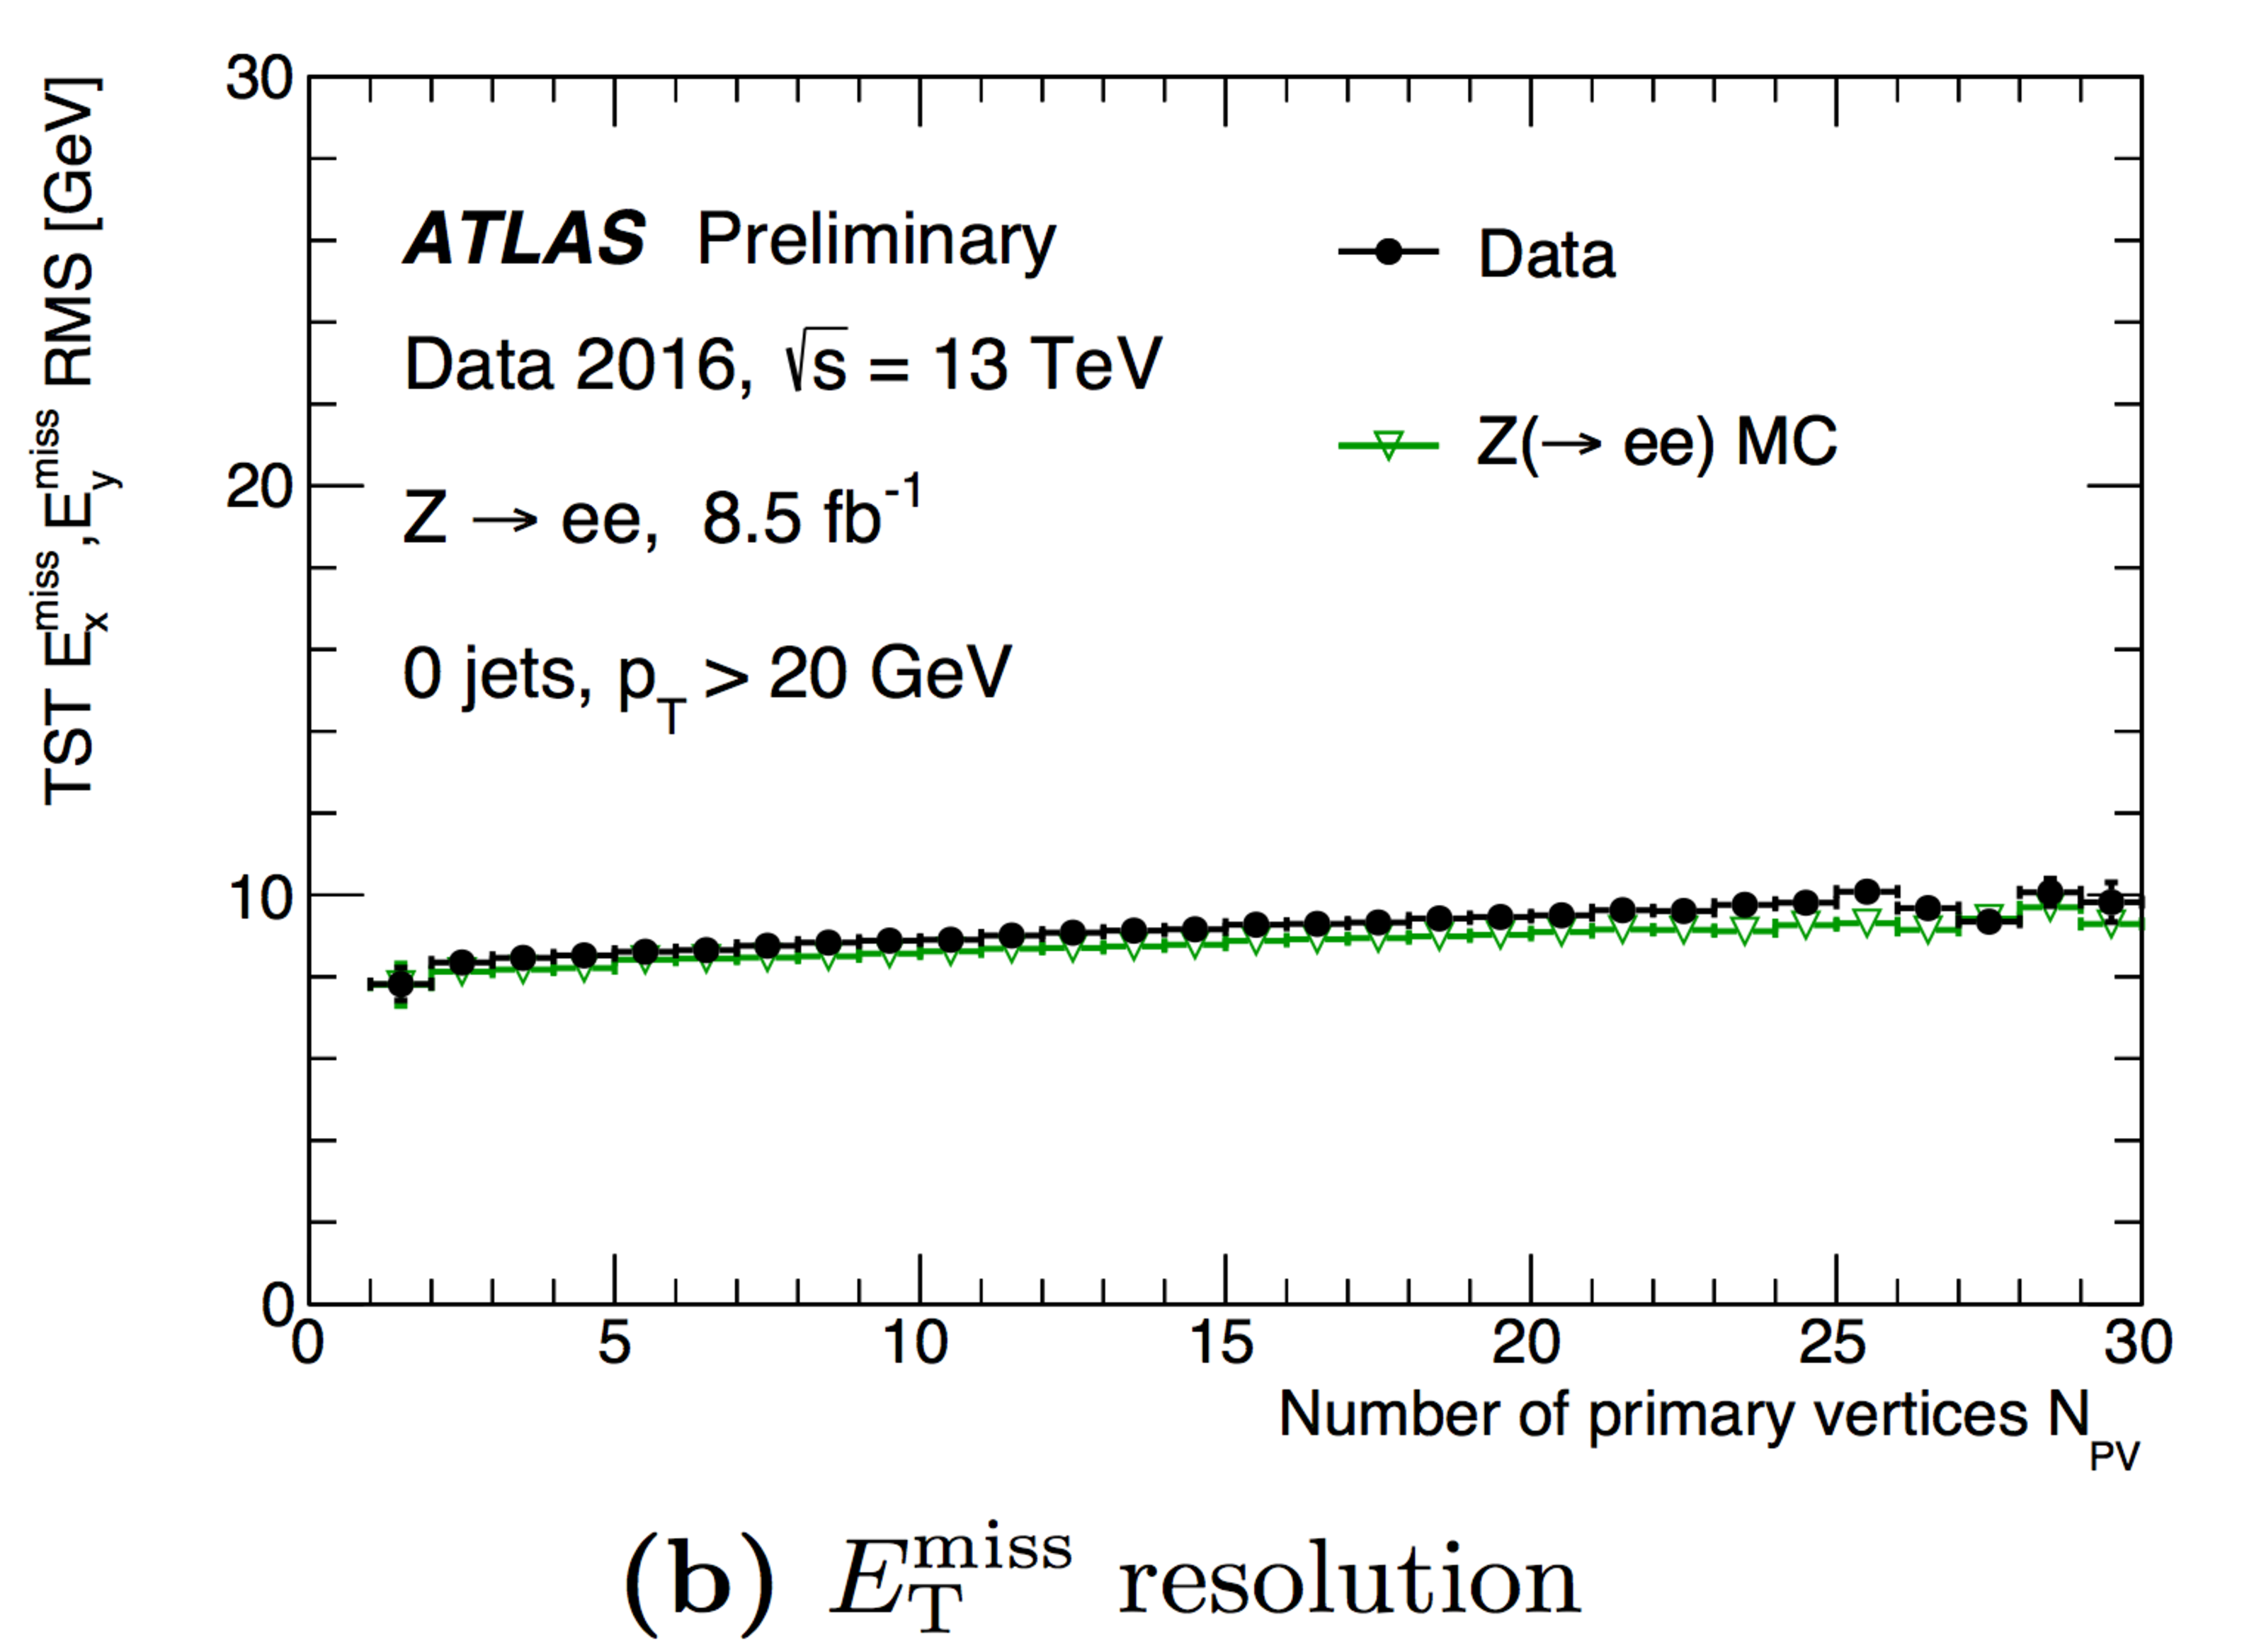
\includegraphics[width=0.48\textwidth]{figures/ObjectDef/metReso_177.pdf}}
    \subfigure[]{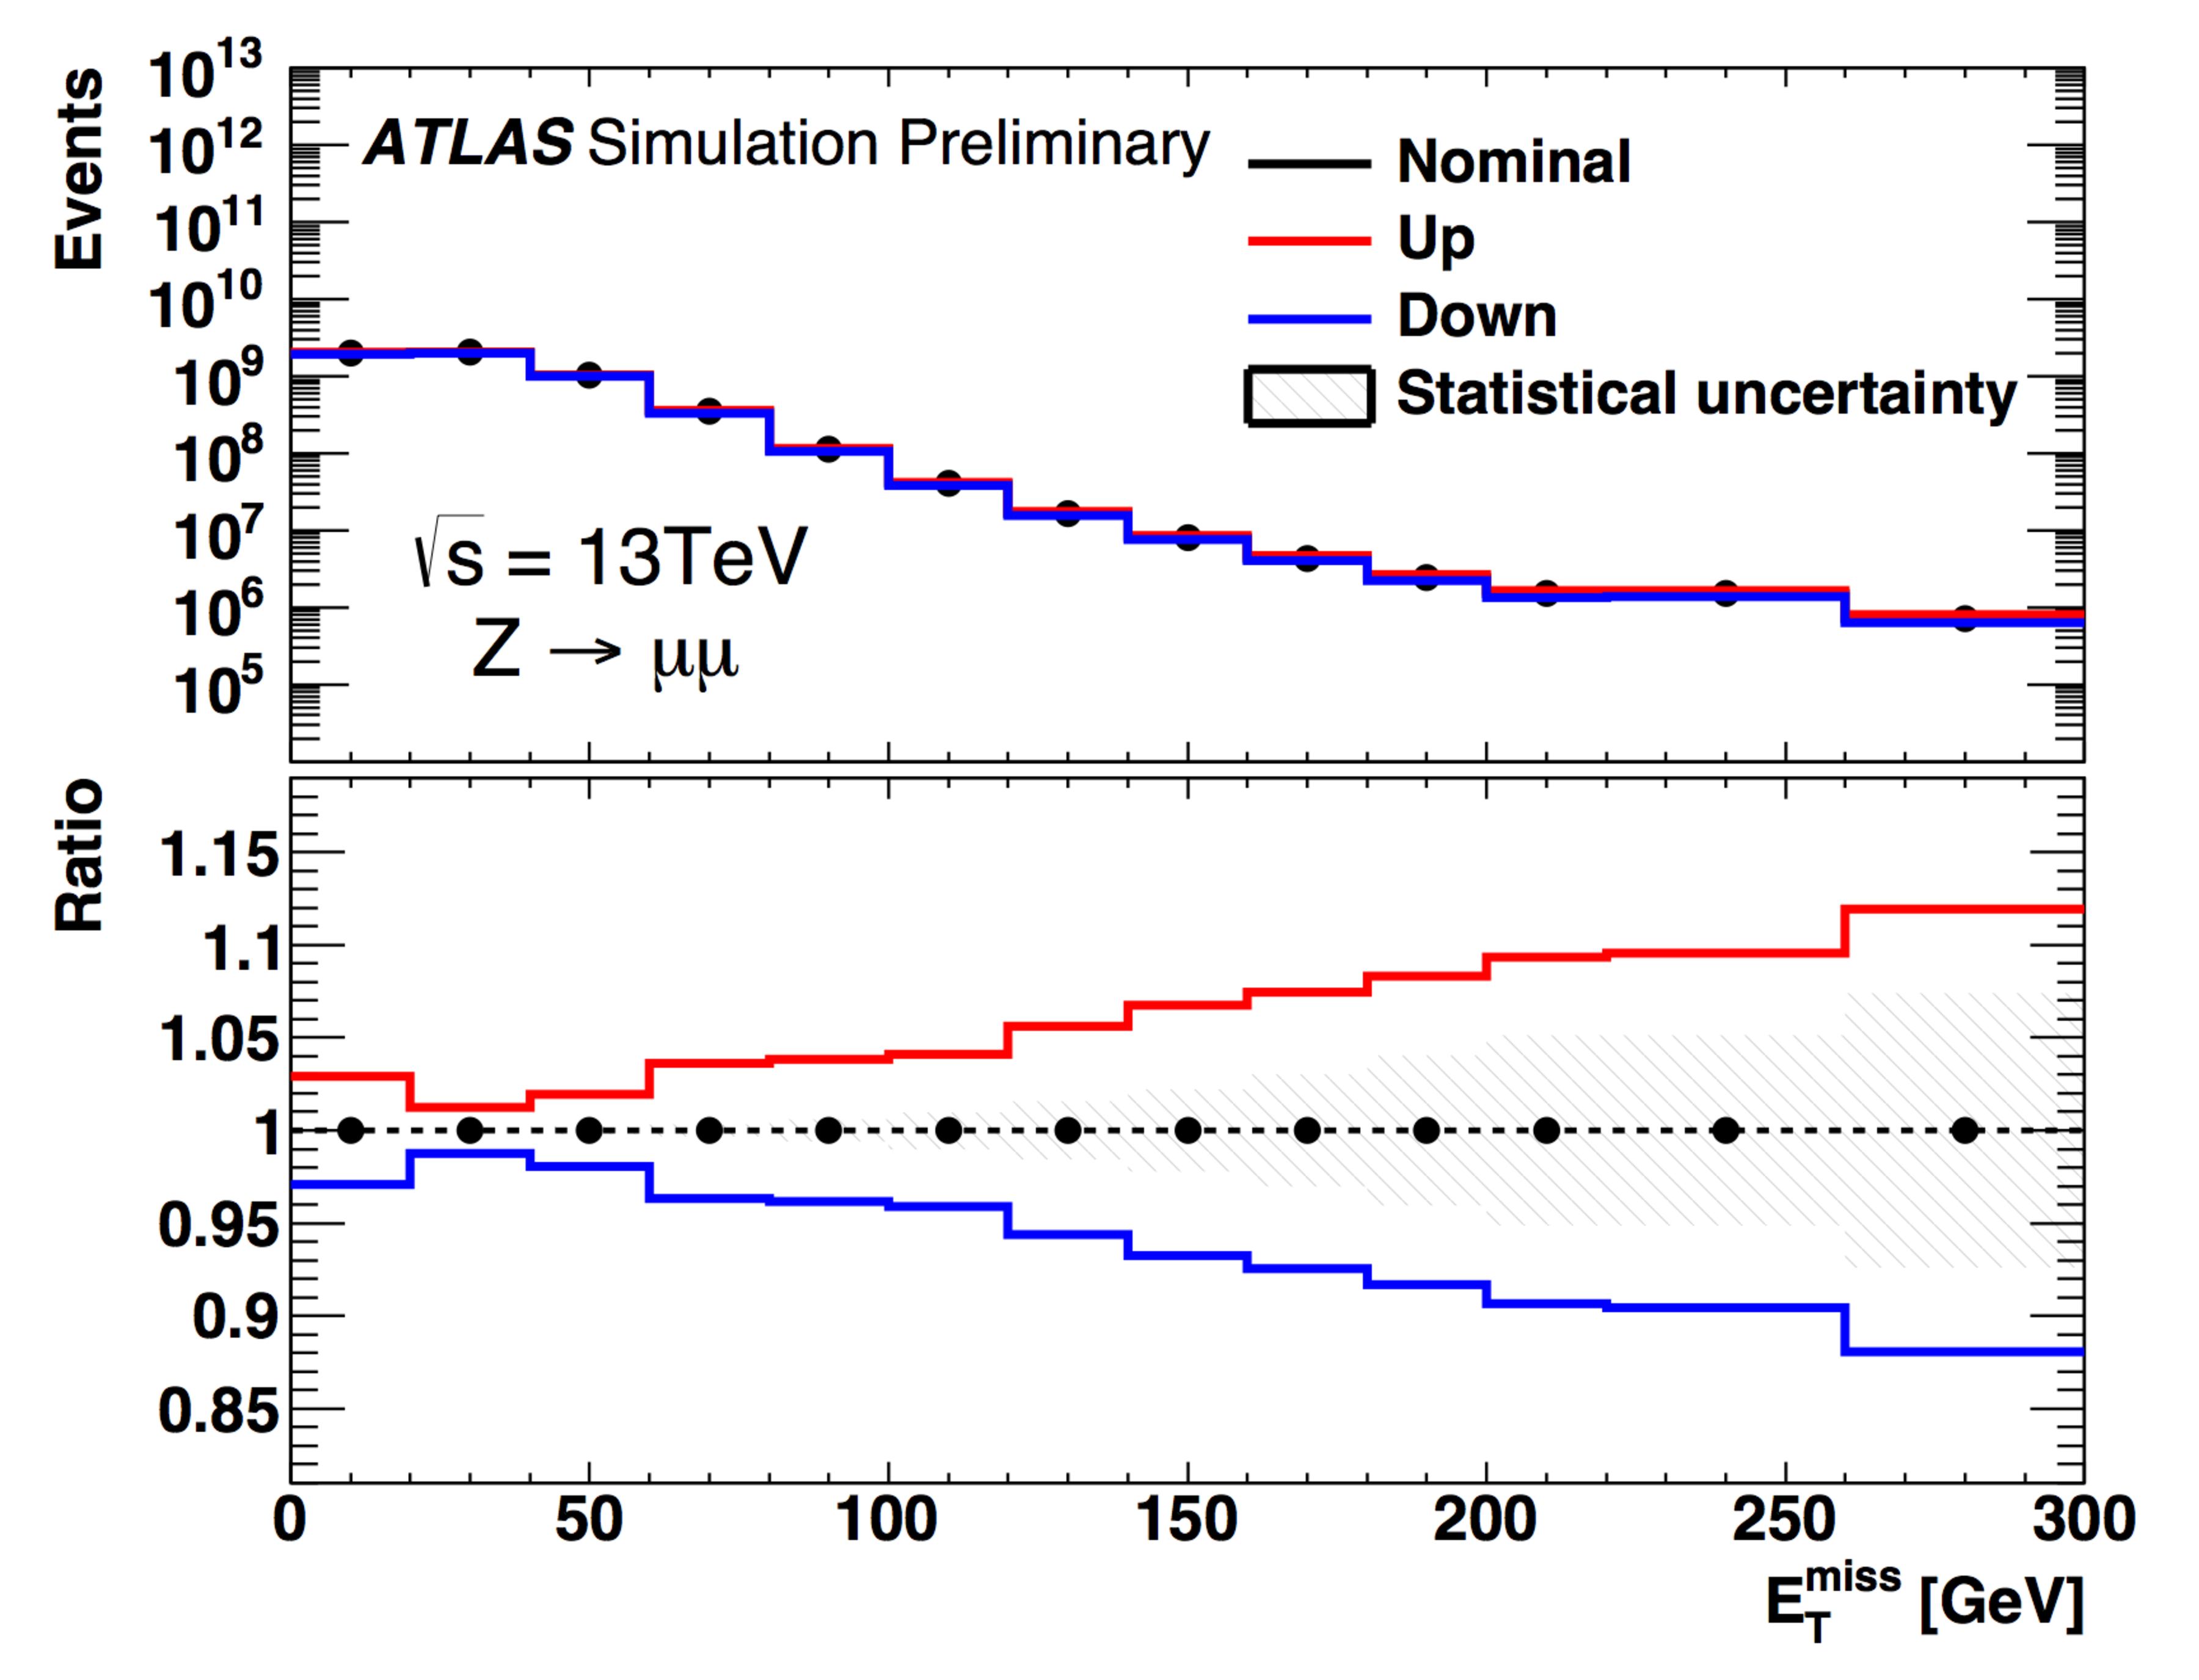
\includegraphics[width=0.48\textwidth]{figures/ObjectDef/metUnct_177.pdf}}
    \caption{ (a) Pile-up dependency of resolution on the met soft term, and (b) the absolute resolution,
      simulated or measured using $Z\ra \ell\ell$ events in which the soft terms is zero with ideal measurement \cite{177_MET_data2016}. 
      \label{fig::objDef::metPerformance}
 }
\end{figure}
%%%%%%%%%%



%%%%%%%%%
\subsection{Object Definition in the Analysis} \label{sec::objDef::objDef}
The requirements for objects used in the analysis is summarized in Table \ref{tab::objDef::summary}.
For electrons and muons, two types of working point are defined;
``baseline'' is the loose selection criteria oriented to veto extra prompt leptons in the event; 
``signal'' is the tighter wokring point aiming to reject fake leptons where the impact parameter cut, isolation requirement and tighter identification are imposed in on top of the baseline requirement.
Signal regions are defined with exactly one baseline and signal lepton, given that the targeted signal events contain exactly one prompt lepton. Jet used in the analysis is uniquely defined. JVT cut is required to avoid the impact by pile-up on the analysis. \\
%% OR通ってないjet使うこともできればいう


\begin{table}[hpt]
\caption{Summary of all baseline and signal object selection. 
In addition to the listed criteria, objects are required to pass the reconstruction, identification and overlap removal.
The $\pt$-threshold is based on the transverse momentum after calibration.
}
\centering
\begin{tabular}{l|l|l}
  \toprule
  \hline
  \textbf{Electrons}	& Baseline			& Signal \\
  \hline
  $p_{T}$		& $p_{T}>7\gev$	                & $p_{T}>10\gev$ \\
  Identification        & Loose \footnote{See Sec. \ref{sec::objDef::electrons::id}} 
        		& Tight \footnote{See Sec. \ref{sec::objDef::electrons::id}} \\
  Isolation		& -				& \texttt{GradientLoose} \\
  Impact parameter cuts & -				& $z_0 < 0.5 \mathrm{mm}$, $|d_0|/\sigma(d_0)<5$ \\

  \hline
  \textbf{Muons}	& Baseline			& Signal \\
  \hline
  $p_{T}$		& $p_{T}>6\gev$	                & $p_{T}>10\gev$ \\
  Identification	& Medium \footnote{See Sec. \ref{sec::objDef::muon::id}} 
                        & Medium \footnote{See Sec. \ref{sec::objDef::muons::id}}  \\
  Isolation		& -				& \texttt{GradientLoose} \\
  Impact parameter cuts & -				& $z_0 < 0.5\mathrm{mm}$, $|d_0|/\sigma(d_0)<3$ \\
  \hline
  \multicolumn{3}{l}{\textbf{Jets}} \\
  \hline
  Clustering Algorithm  & \multicolumn{2}{l}{\Antikt ($r=0.4$)}  \\
  $p_{T}$		& \multicolumn{2}{l}{$p_{T}>30\gev$}  \\
    JVT			& \multicolumn{2}{l}{JVT$>0.57$} 	 \\
  $b$-tag	        & \multicolumn{2}{l}{MV2c10 77\% efficiency working point} \\
  \hline
\end{tabular}
\label{tab::objDef::summary}
\end{table}

